%%%%%%%%%%%%%%%%%%%%%%%%%%%%%%%%%%%%%%%%%%%%%%%%%%%%%%%%%%%%%%%
%
% University of Milano Bicocca
% Software engineering project
% Developed by
% 
% 
% Tasca Alessandro 845150
% Lenzini Giacomo 851626
% Bonfanti Samuele 851656
% Dedo' Shana 851660
% 
%
%%%%%%%%%%%%%%%%%%%%%%%%%%%%%%%%%%%%%%%%%%%%%%%%%%%%%%%%%%%%%%%

\documentclass[12pt]{article}

% Language setting
\usepackage[italian]{babel}

% Set page size and margins
% Replace `letterpaper' with`a4paper' for UK/EU standard size
\usepackage[letterpaper,top=2cm,bottom=2cm,left=3cm,right=3cm,marginparwidth=1.75cm]{geometry}

% Useful packages
\usepackage{float}
\usepackage{amsmath}
\usepackage{graphicx}
\usepackage[colorlinks=true, allcolors=black]{hyperref}


\title{
  Brew Day! \\ 
  \large Ingengeria del Software \\
    aa 2021-2022}

\author{Tasca Alessandro, Lenzini Giacomo, Bonfanti Samuele, Dedo' Shana}

\date{31 Gennaio 2022}

\begin{document}

\maketitle
\newpage


\tableofcontents
\newpage
\section{Organizzazione}

\subsection{Diagramma di Gantt}

\subsubsection{Iniziale}
\begin{figure}[H]
\centering
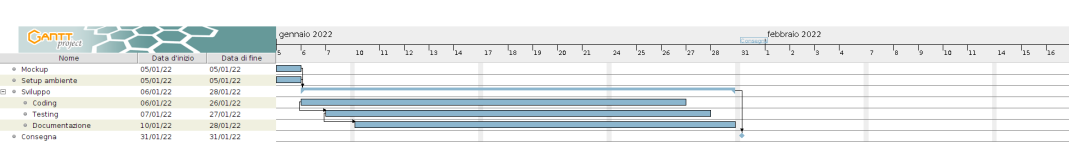
\includegraphics[width=440px]{gantt_iniziale.png}
\caption{\label{fig:gantt_iniziale}Diagramma di Gantt a inizio progetto}
\end{figure}

\subsubsection{Finale}
\begin{figure}[H]
\centering
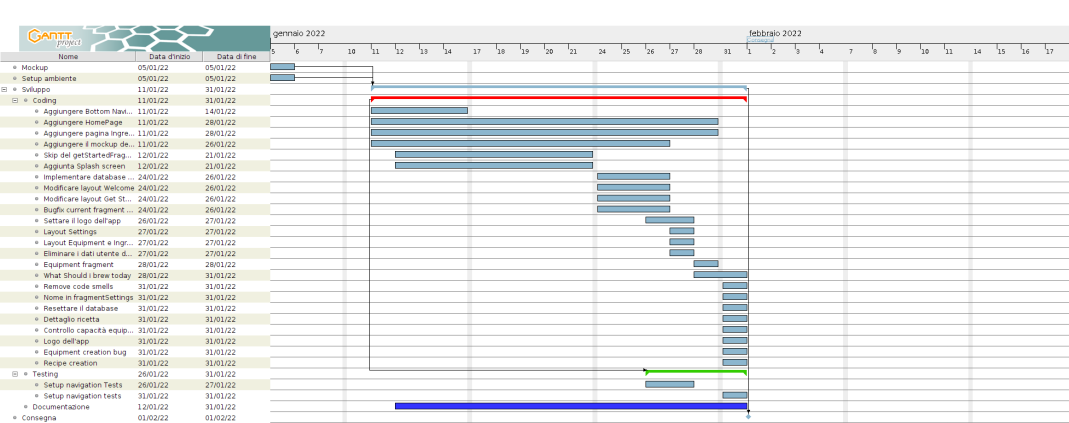
\includegraphics[width=440px]{gantt_finale.png}
\caption{\label{fig:gantt_finale}Diagramma di Gantt a fine progetto}
\end{figure}
%%%%%%%%%%%%%%%%%%%%%%%%%%%%%%%%%%%%%%%%%%%%%%%%%%%%%%%%%%%%%%%%%%%%%%%%%%%%%%%%%%%%%%%%%%%%%%%%%%%%%%%%%%
\newpage
\section{Analisi}


\subsection{Requisiti Funzionali}

\begin{table}[H]
\centering
\begin{tabular}{l|p{10cm}}
Tipo & Descrizione \\
\hline\hline
Funzionale & Mantenimento lista ingredienti \\\hline
Funzionale & Aggiornamento lista ingredienti in base agli acquisti effettuati dall’utente \\\hline
Funzionale & Aggiornamento lista in base ai consumi effettuati dall’utente per produrre una determinata ricetta \\\hline
Funzionale & Mantenimento di una lista di ricette \\\hline
Funzionale & Supporto creazione, modifica e cancellazione di ricette \\\hline
Funzionale & Supporto creazione di note su ricette \\\hline
Funzionale & Implementazione feature “What should I brew today?” \\\hline
Funzionale & Le ricette devono essere soltanto di tipo “all grain” \\\hline
Funzionale & L’equipaggiamento ha una specifica “batch size” (il max. numero di litri per singola run) \\\hline
Funzionale & Le ricette possono contenere solo acqua, malto, luppolo, lievito, zucchero, additivi\\ \hline
Funzionale & Mantenimento cronologia delle ricette svolte con relative note di produzione \\\hline
Funzionale & Mantenimento dati sulla capacità della strumentazione dell’utente \\
\end{tabular}
\caption{\label{tab:tabella_requisiti}Tabella riassuntiva dei requisiti identificati}
\end{table}


\subsection{Attori}

\begin{table}[H]
\centering
\begin{tabular}{l|p{6cm}}
Attore & Obiettivo \\
\hline\hline
Utente & CURD ricette \newline
aggiungere ingredienti \newline
aggiungere equipaggiamento \\
\end{tabular}
\caption{\label{tab:tabella_attori}Tabella riassuntiva attori}
\end{table}


\subsection{Casi d'uso}

\begin{table}[H] %H parameter prevents from reposition (preamble:\usepackage{float})

\centering
\begin{tabular}{l|p{10cm}}%allign left = l, right = r, center = c, p = automatic new line
Caso d'uso & Descrizione \\
\hline\hline
RegistrazioneUtente & L'attore Utente deve registrarsi con il nome in modo da poter utilizzare l'app \\
\hline
ModficaUtente & L'attore Utente può modificare i propri dati(nome) \\
\hline
EliminazioneUtente & L'attore Utente può eliminare i propri dati dall'app \\
\hline
AggiungiRicetta & L'attore Utente può creare una ricetta nel sistema \\
\hline
ModificaRicetta & L'attore Utente può modificare i dettagli relativi a una ricetta presente nel sistema \\
\hline
EliminaRicetta & L'attore Utente può eliminare una ricetta dal sistema \\
\hline
VisualizzaCronologia & L'attore Utente può visualizzare l'elenco della cronologia di utilizzo di una singola ricetta e delle sue note \\
\hline
VisualizzaRicetta & L'attore Utente può visualizzare le ricette presenti del sistema \\
\hline
AggiungiIngrediente & L'attore Utente può aggiungere un ingrediente nel sistema \\
\hline
AggiungiEquipaggiamento & L'attore Utente può aggiungere un equipaggiamento nel sistema \\
\hline
WhatShouldIbrewToday? & L'attore Utente può chiedere al sistema di proportgli una ricetta da realizzare massimizzando gli ingredienti disponibili \\
\end{tabular}
\caption{\label{tab:tabella_casi_d_uso}Tabella riassuntiva casi d'uso}
\end{table}


\subsubsection{Diagramma dei casi d'uso}

\begin{figure}[H]
\centering
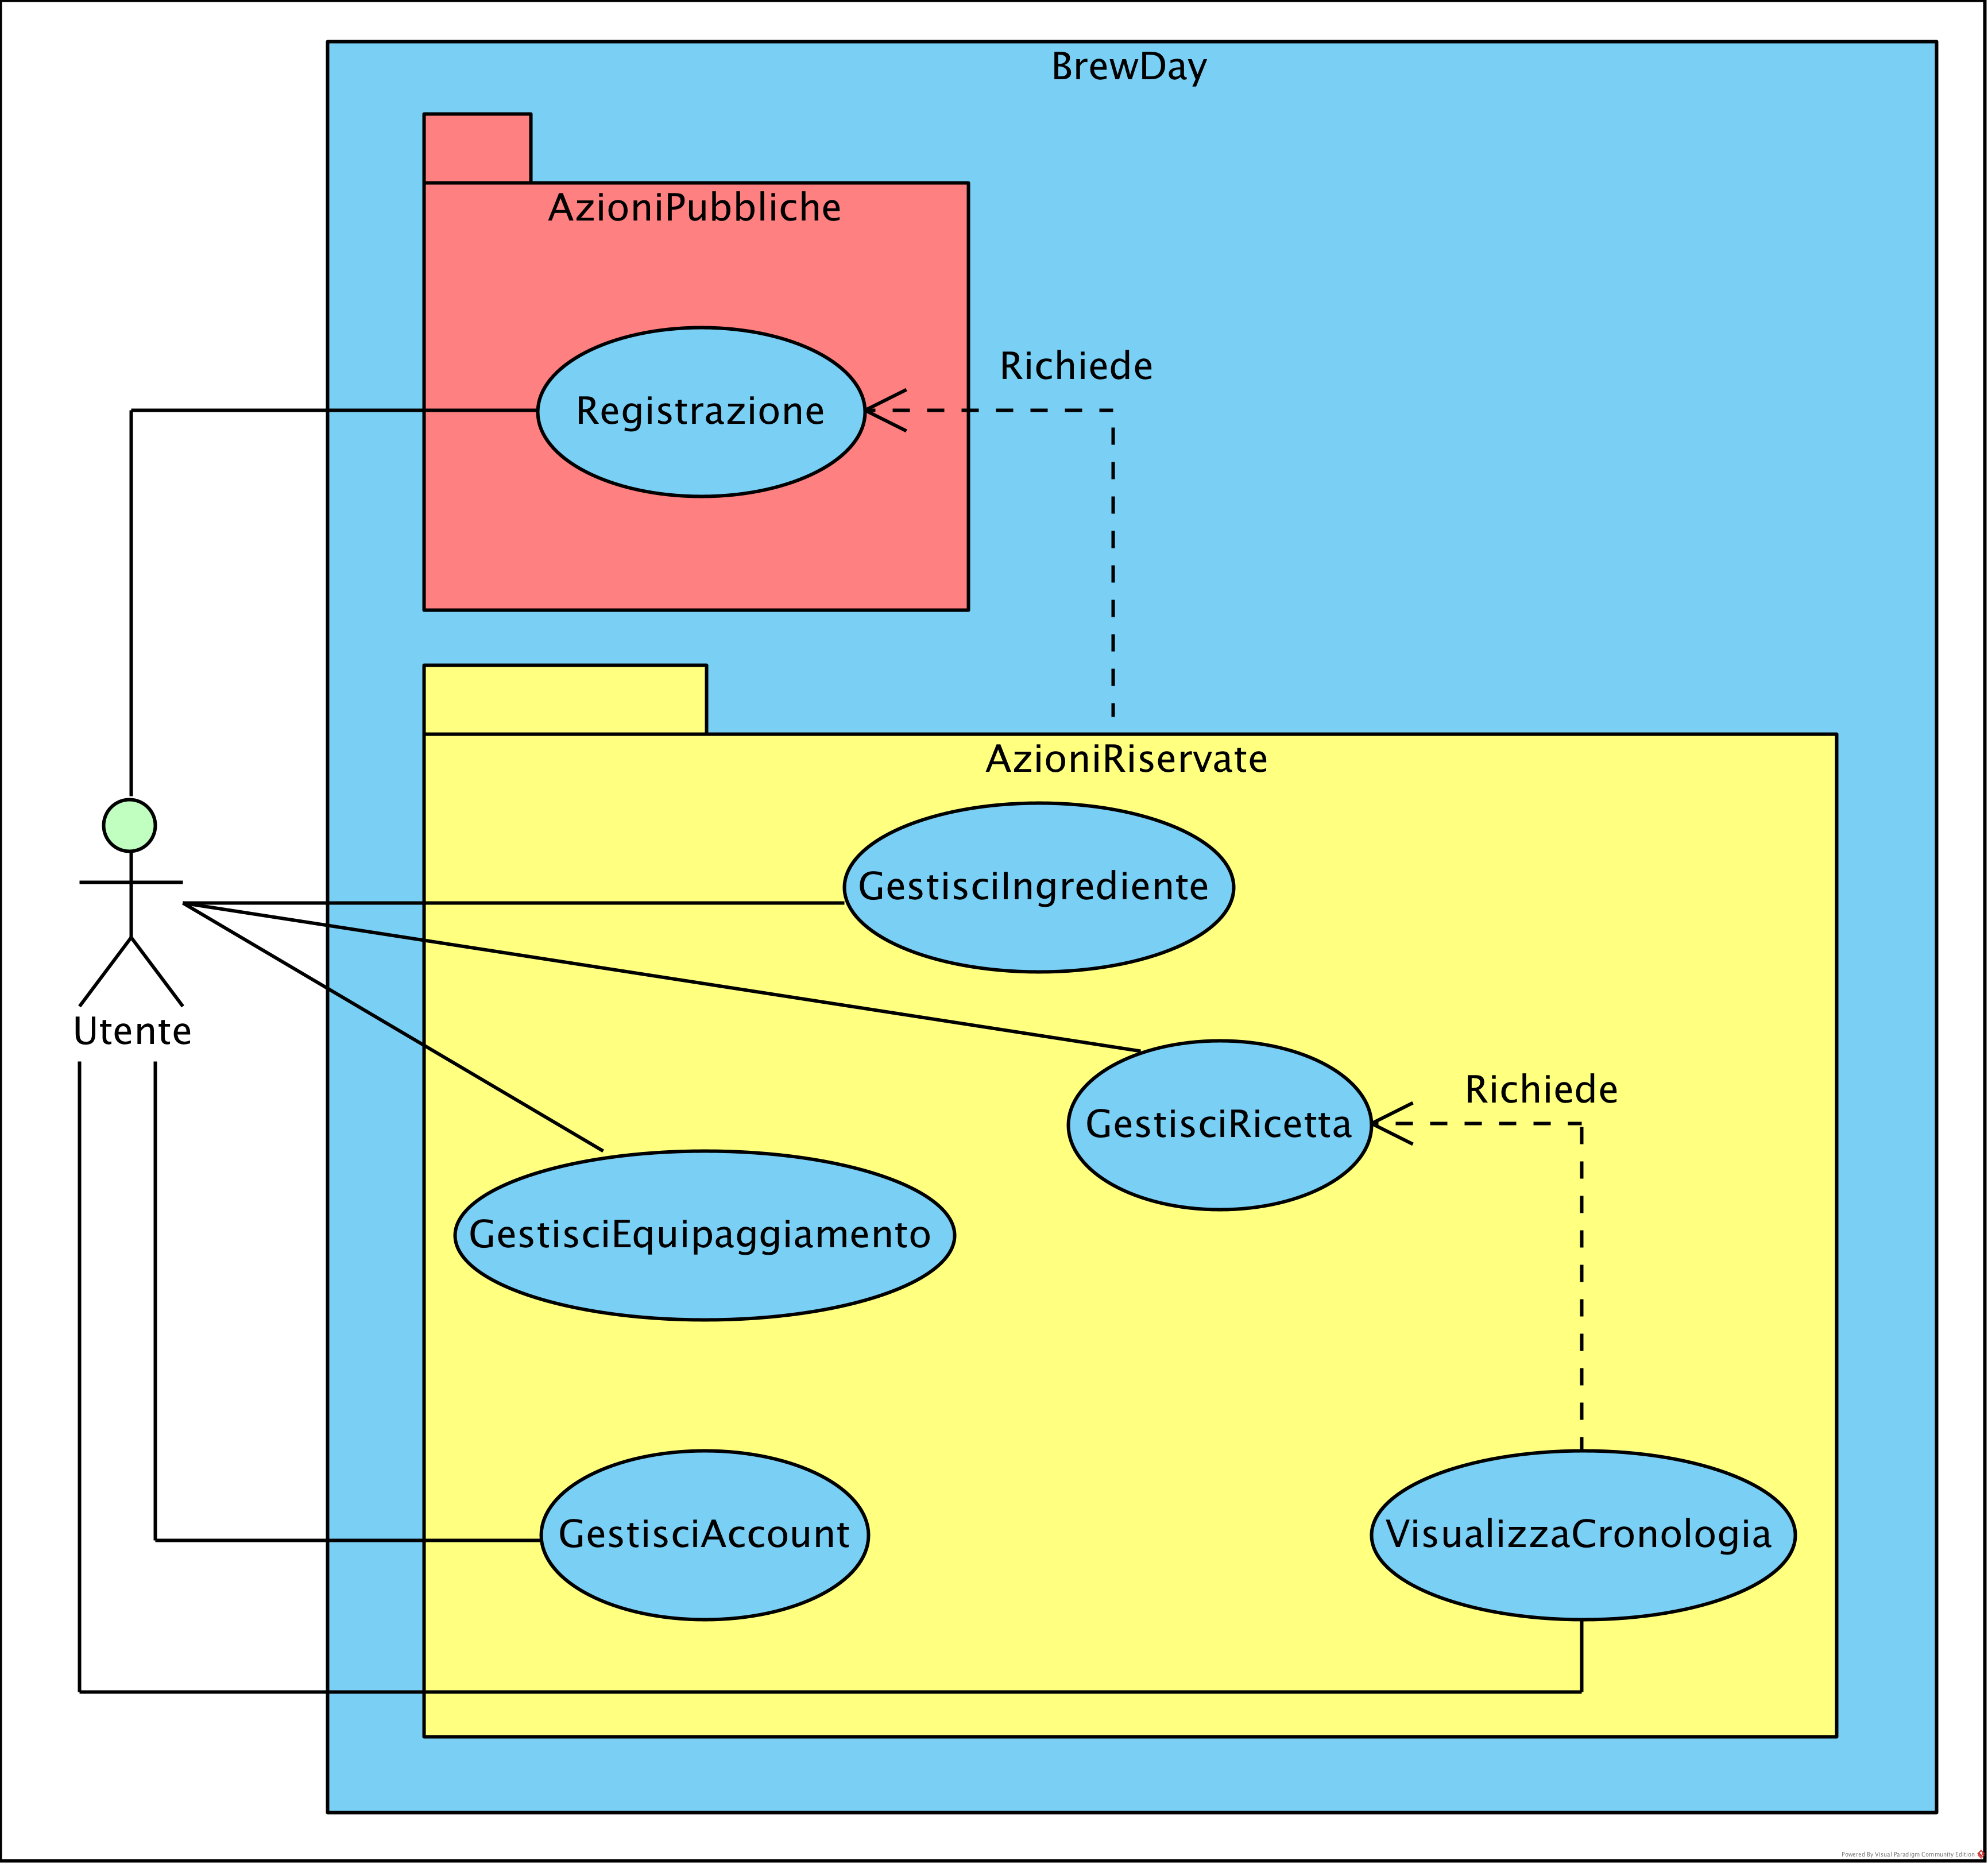
\includegraphics[width=440px]{diagramma_casi_d_uso.png}
\caption{\label{fig:diagramma_casi_d_uso}Diagramma dei casi d'uso}
\end{figure}


\subsection{Modello di Dominio}

\begin{figure}[H]
\centering
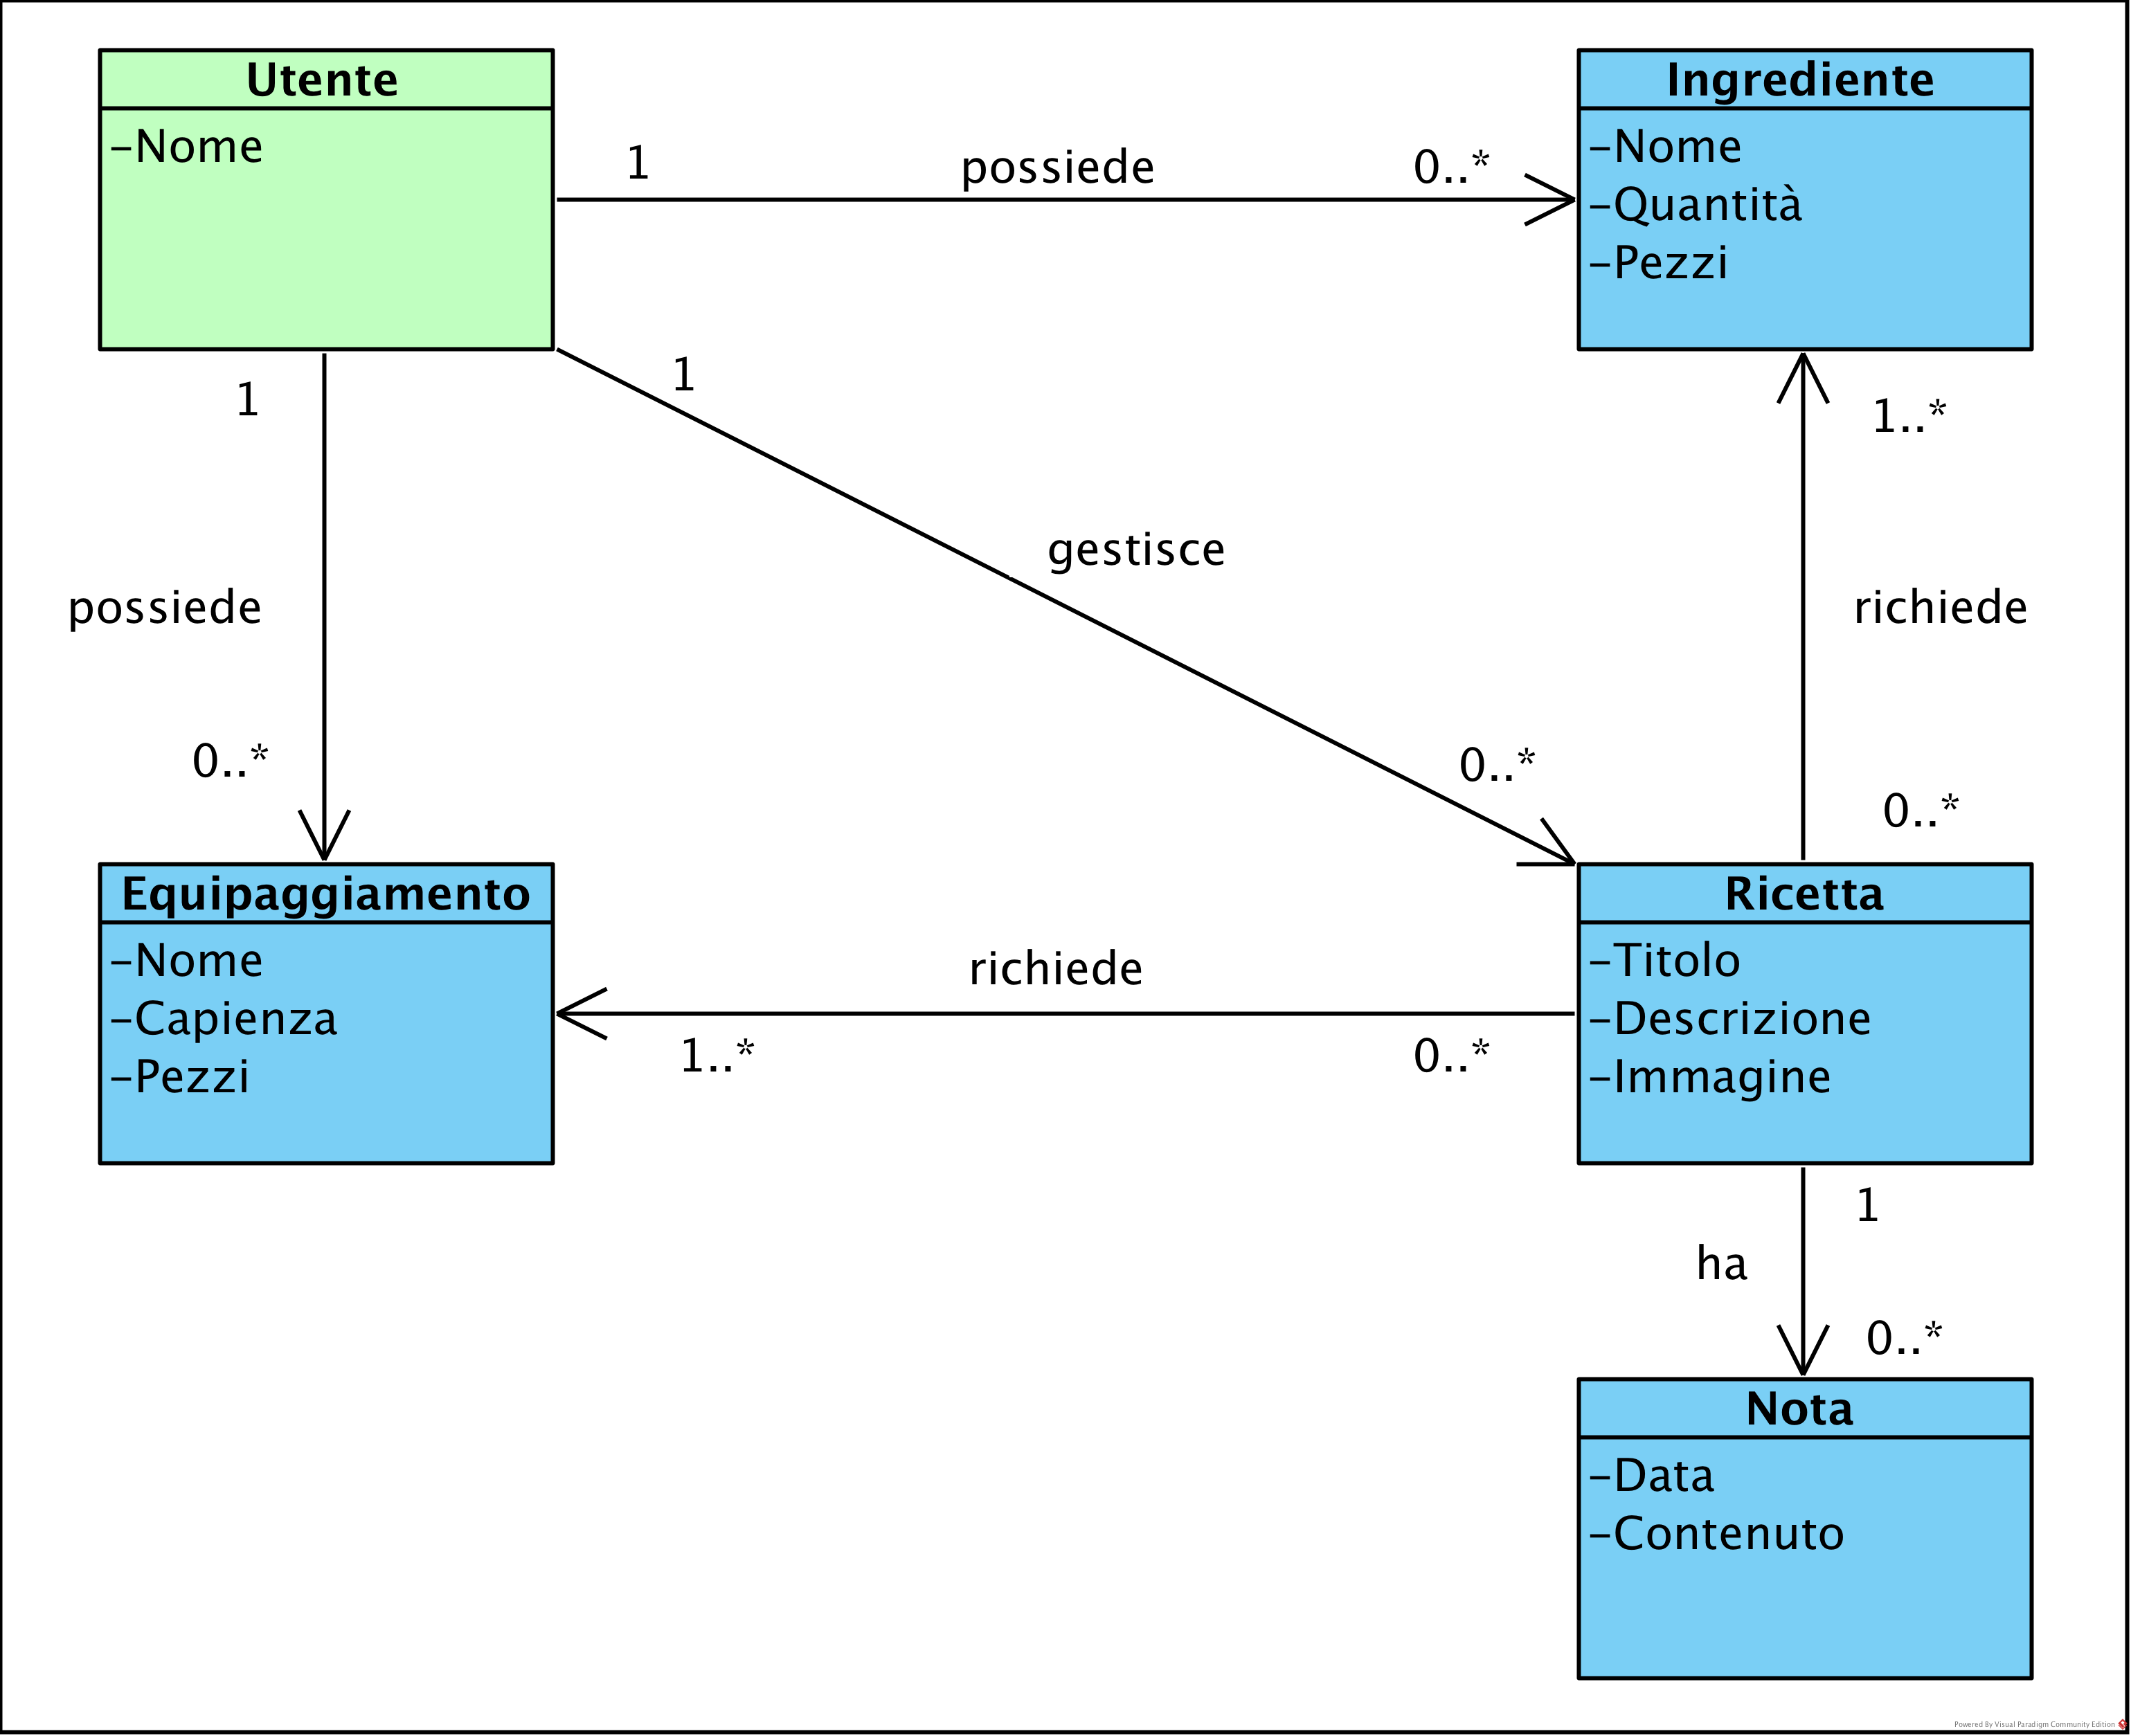
\includegraphics[width=440px]{modello_dominio.png}
\caption{\label{fig:modello_dominio}Modello di Dominio}
\end{figure}

\subsection{Diagramma di sequenza di sistema}
\begin{figure}[H]
\centering
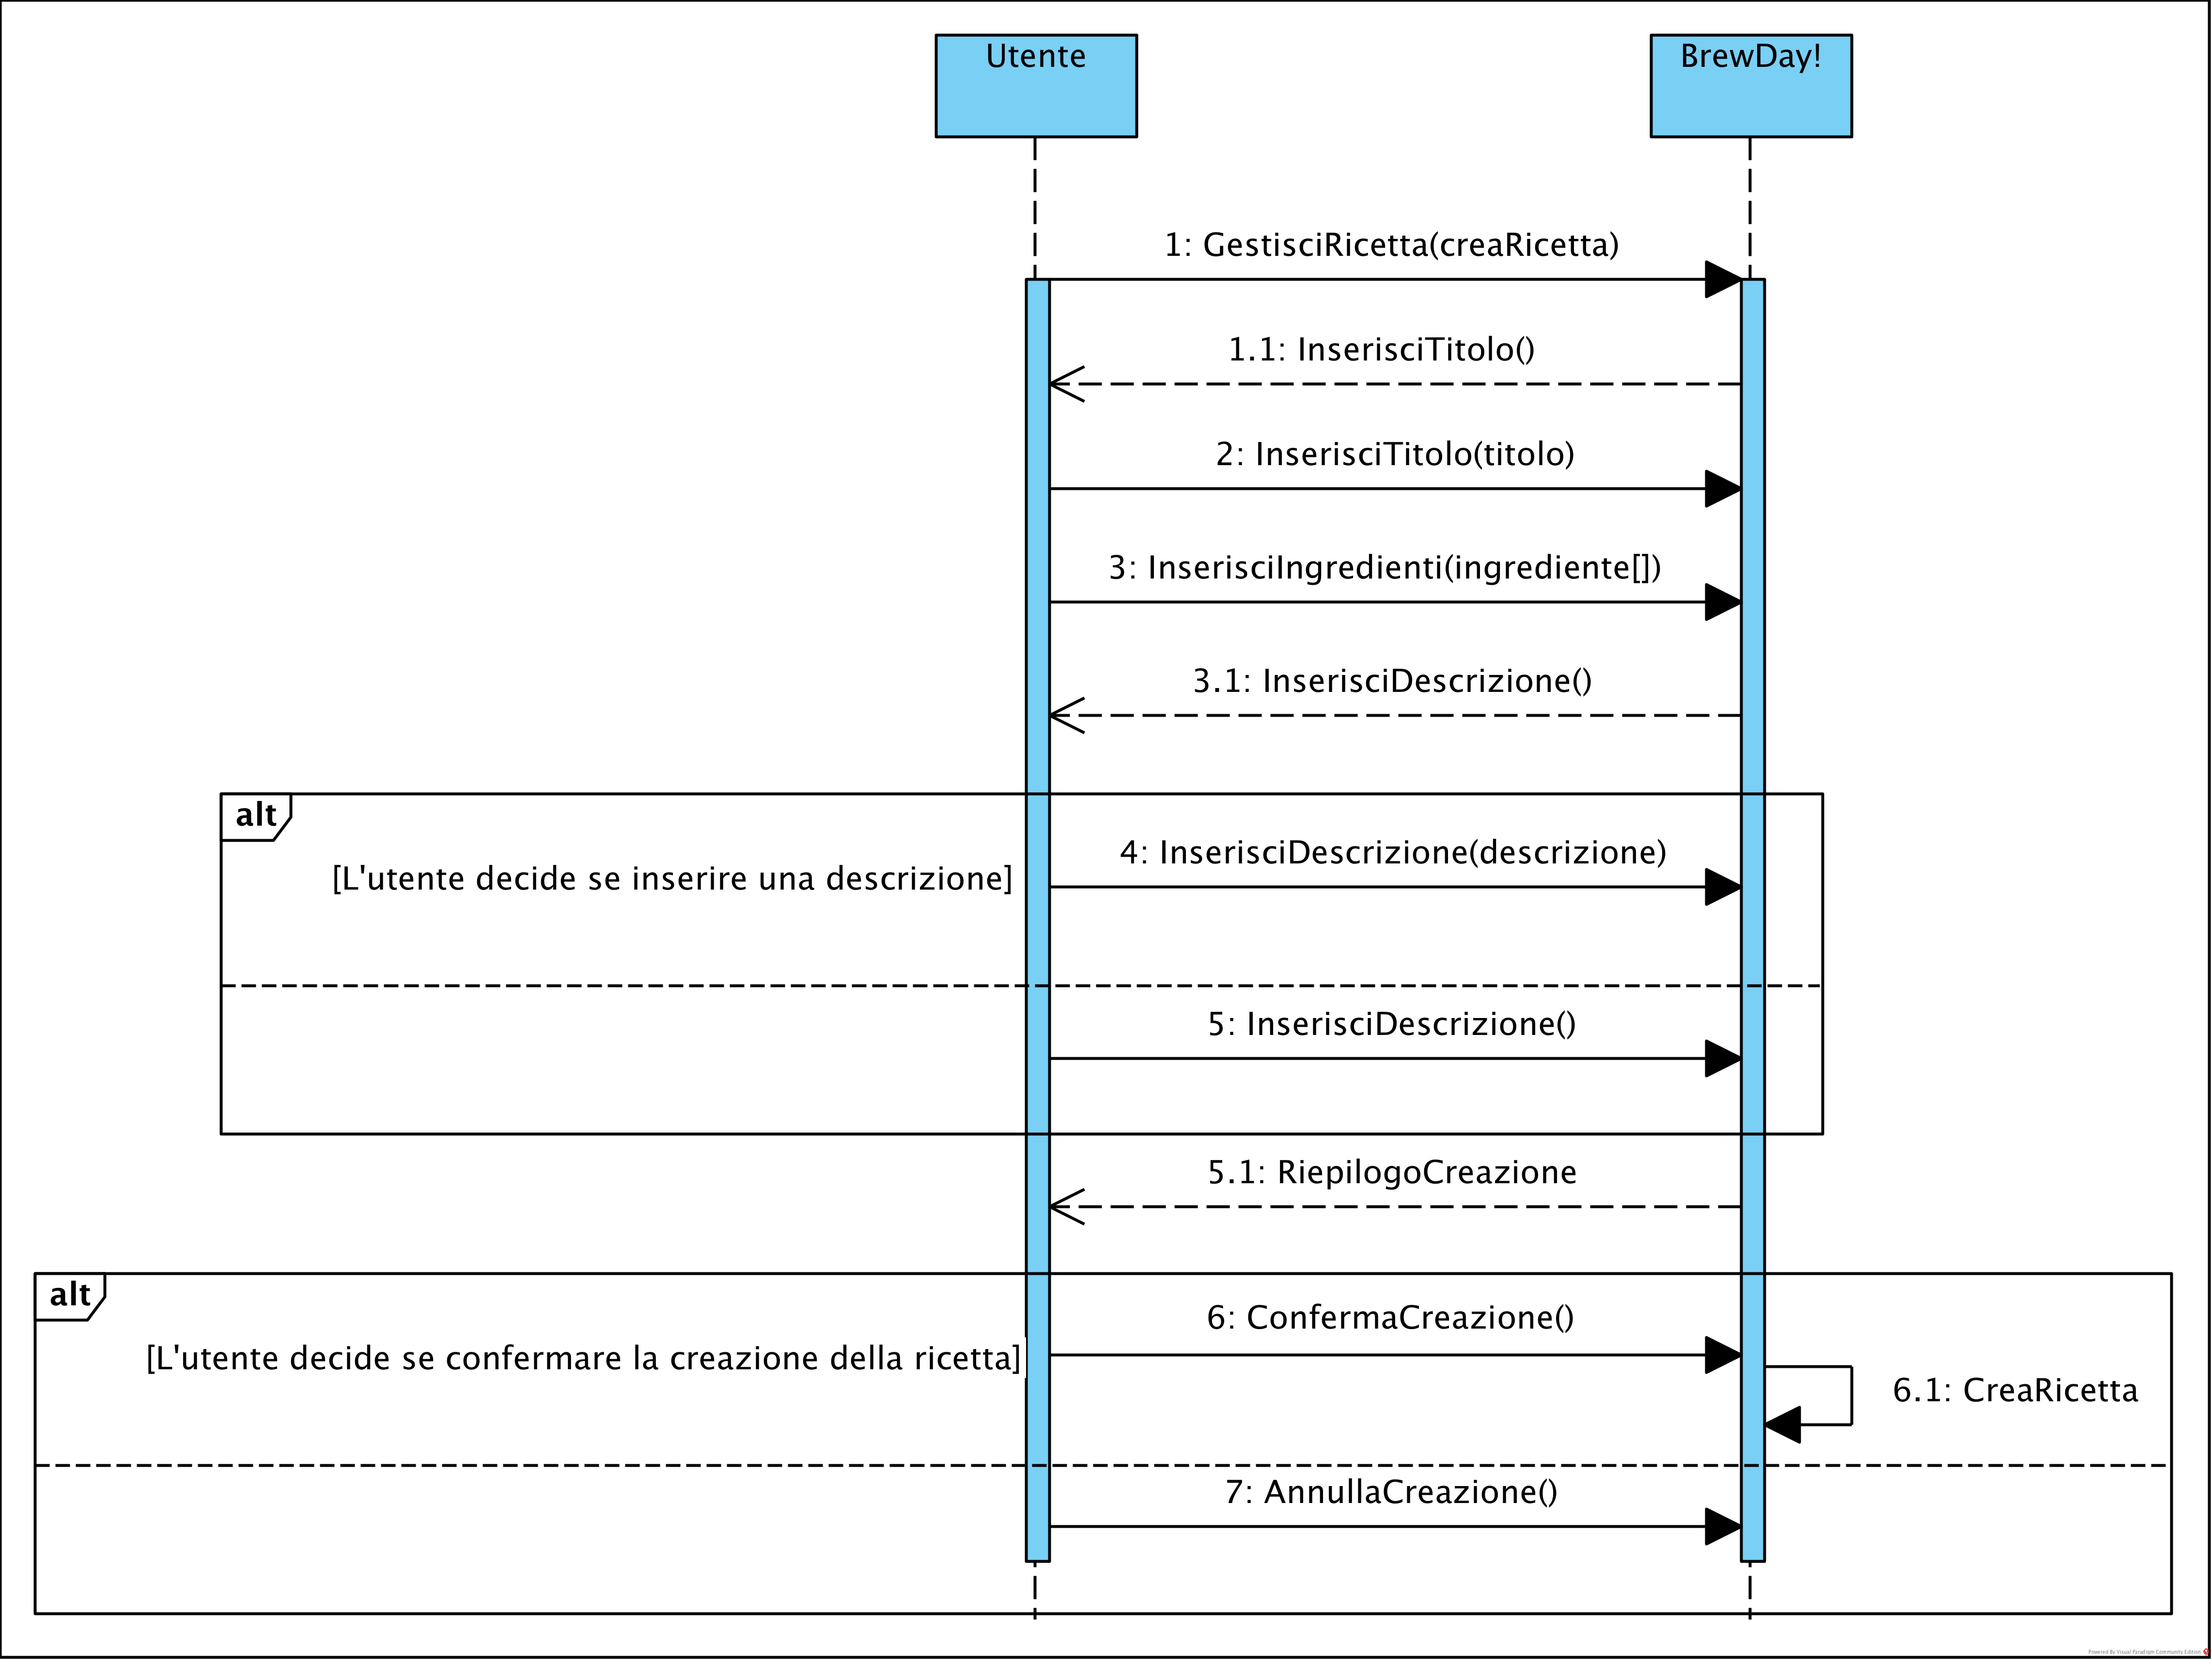
\includegraphics[width=440px]{SSD_addRecipe.png}
\caption{\label{fig:ssd_addRecipe}Diagramma di sequenza di sistema per addRecipe}
\end{figure}

%%%%%%%%%%%%%%%%%%%%%%%%%%%%%%%%%%%%%%%%%%%%%%%%%%%%%%%%%%%%%%%%%%%%%%%%%%%%%%%%%%%%%%%%%%%%%%%%%%%%%%%%%
\newpage
\section{Progettazione}

\subsection{Modello E-R database}
\begin{figure}[H]
\centering
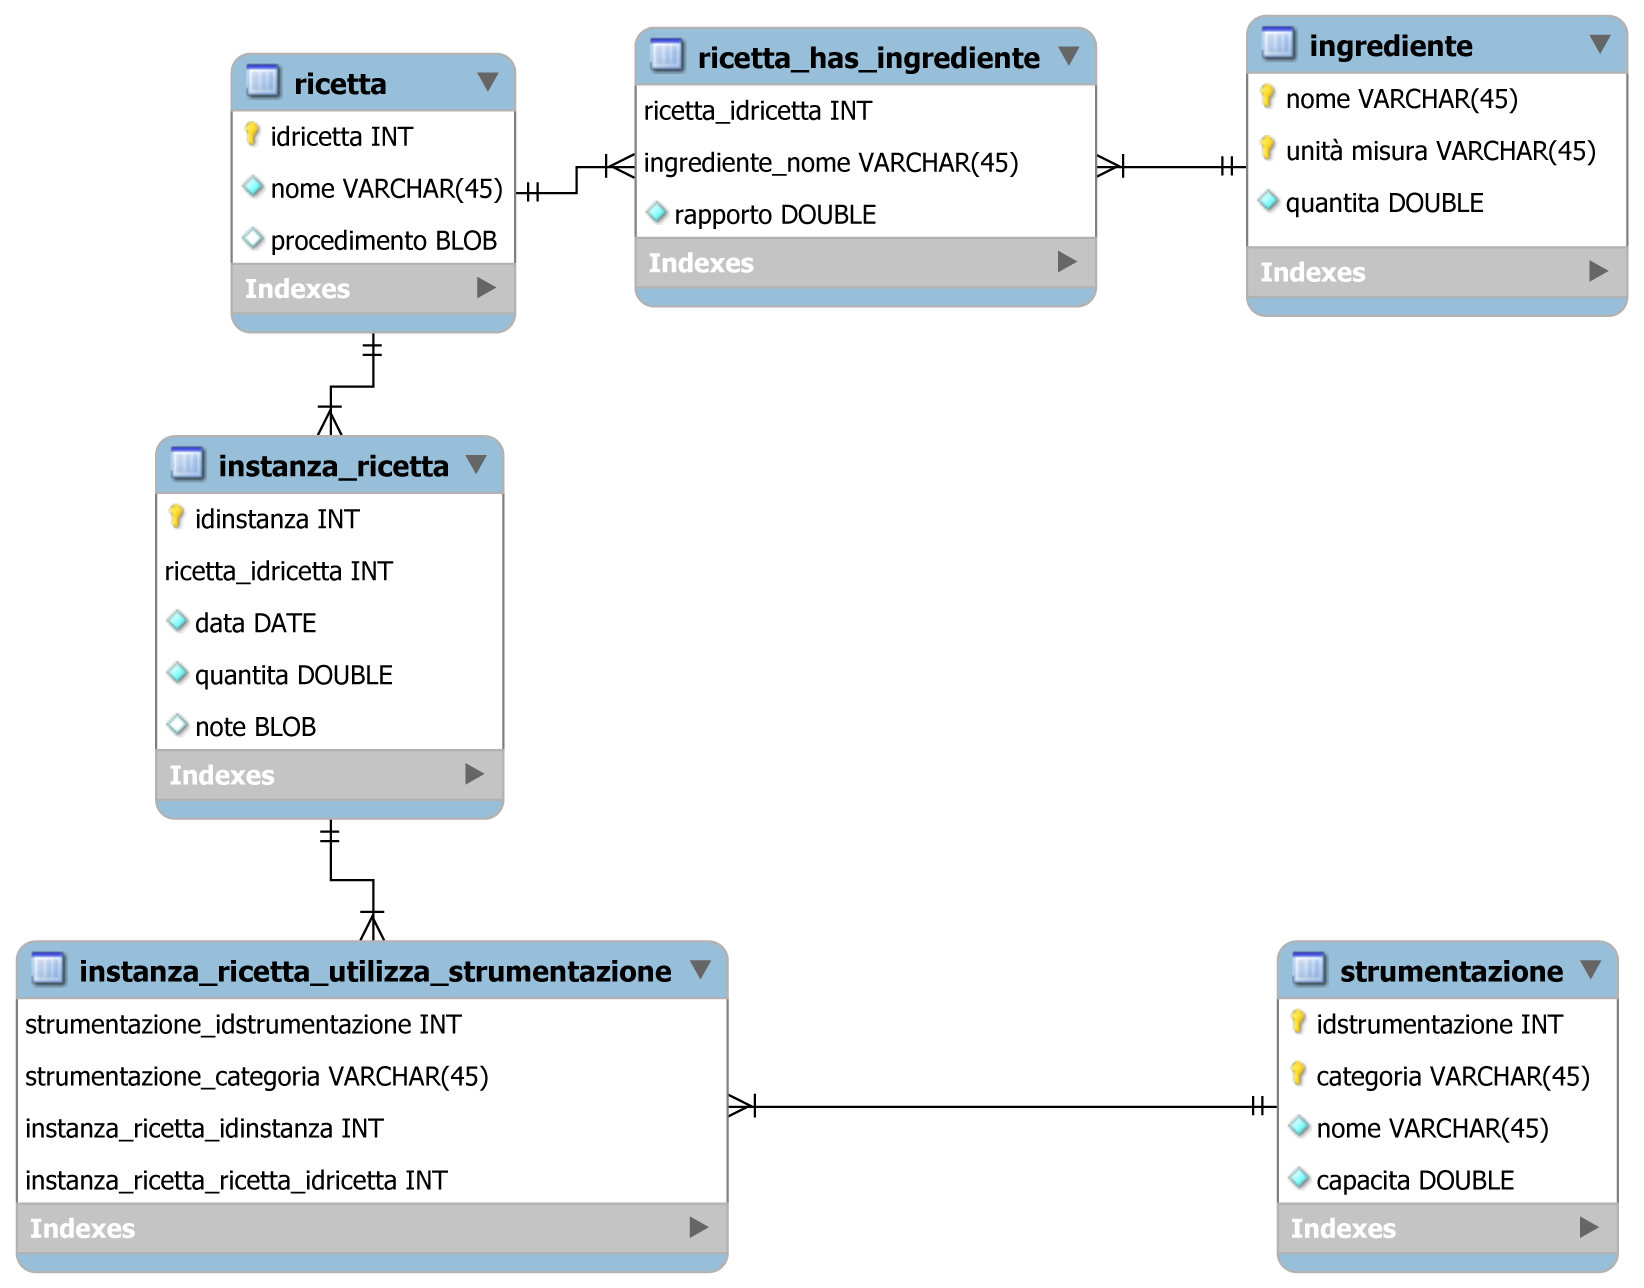
\includegraphics[width=440px]{modello_e_r.png}
\caption{\label{fig:modello_e_r}Modello E-R raffigurante la struttura del database}
\end{figure}



\subsection{Diagramma delle classi}
\begin{figure}[H]
\centering
\includegraphics[width=440px]{diagramma_classi.png}
\caption{\label{fig:diagramma_delle_classi}Diagramma delle classi}
\end{figure}


\subsection{Diagramma di sequenza}
\begin{figure}[H]
\centering
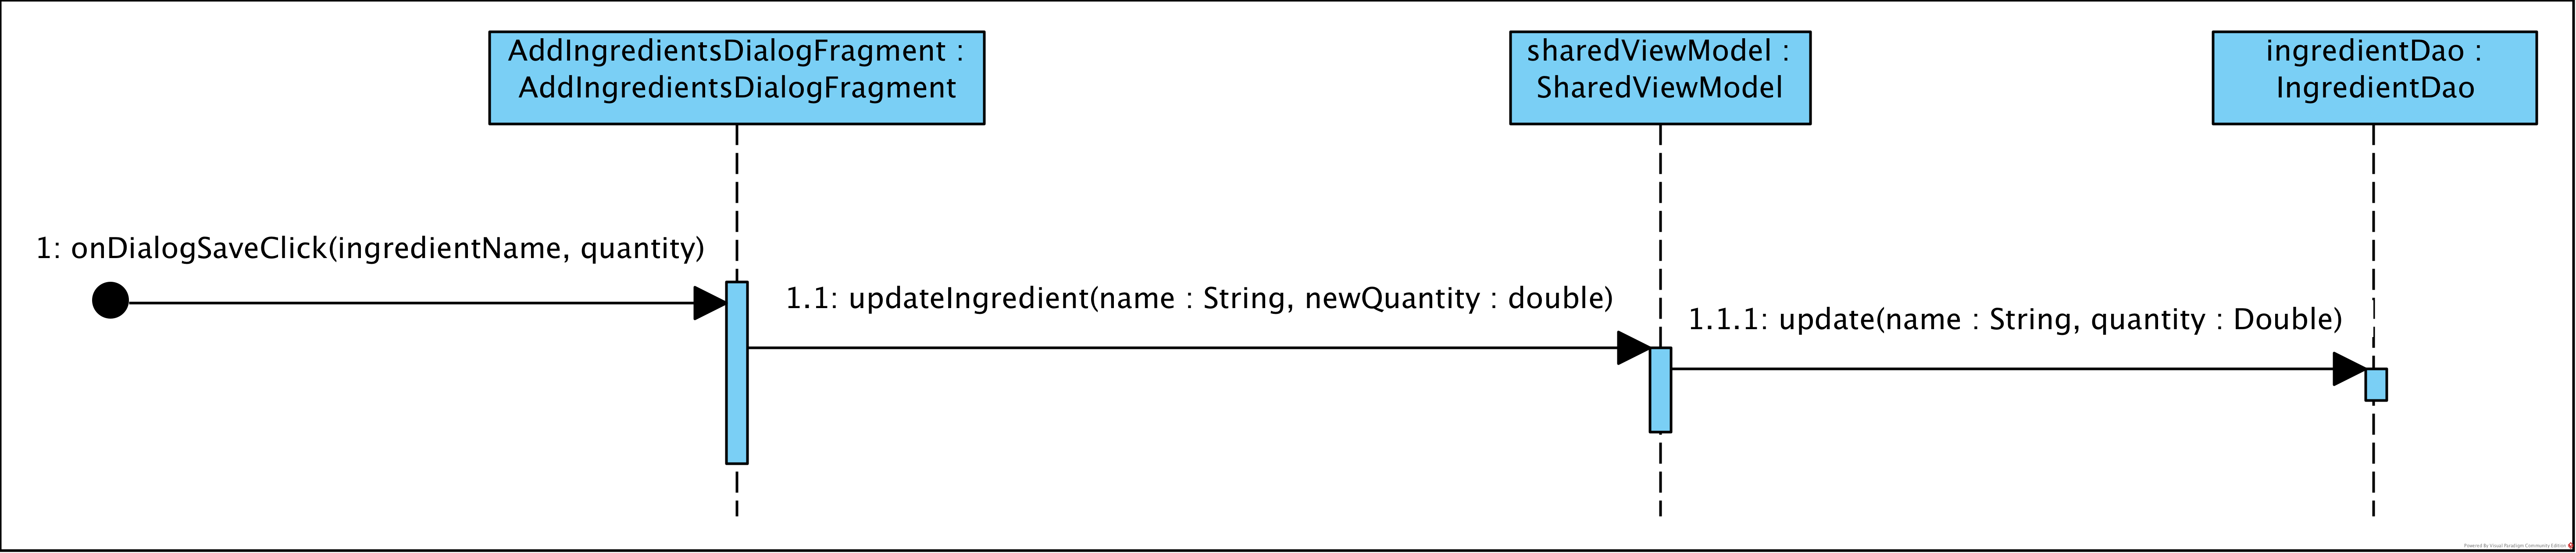
\includegraphics[width=440px]{SD_addIngredient.png}
\caption{\label{fig:diagramma_di_sequenza}Diagramma di sequenza per addIngredient}
\end{figure}


\subsection{Diagramma macchina a stati}
\begin{figure}[H]
\centering
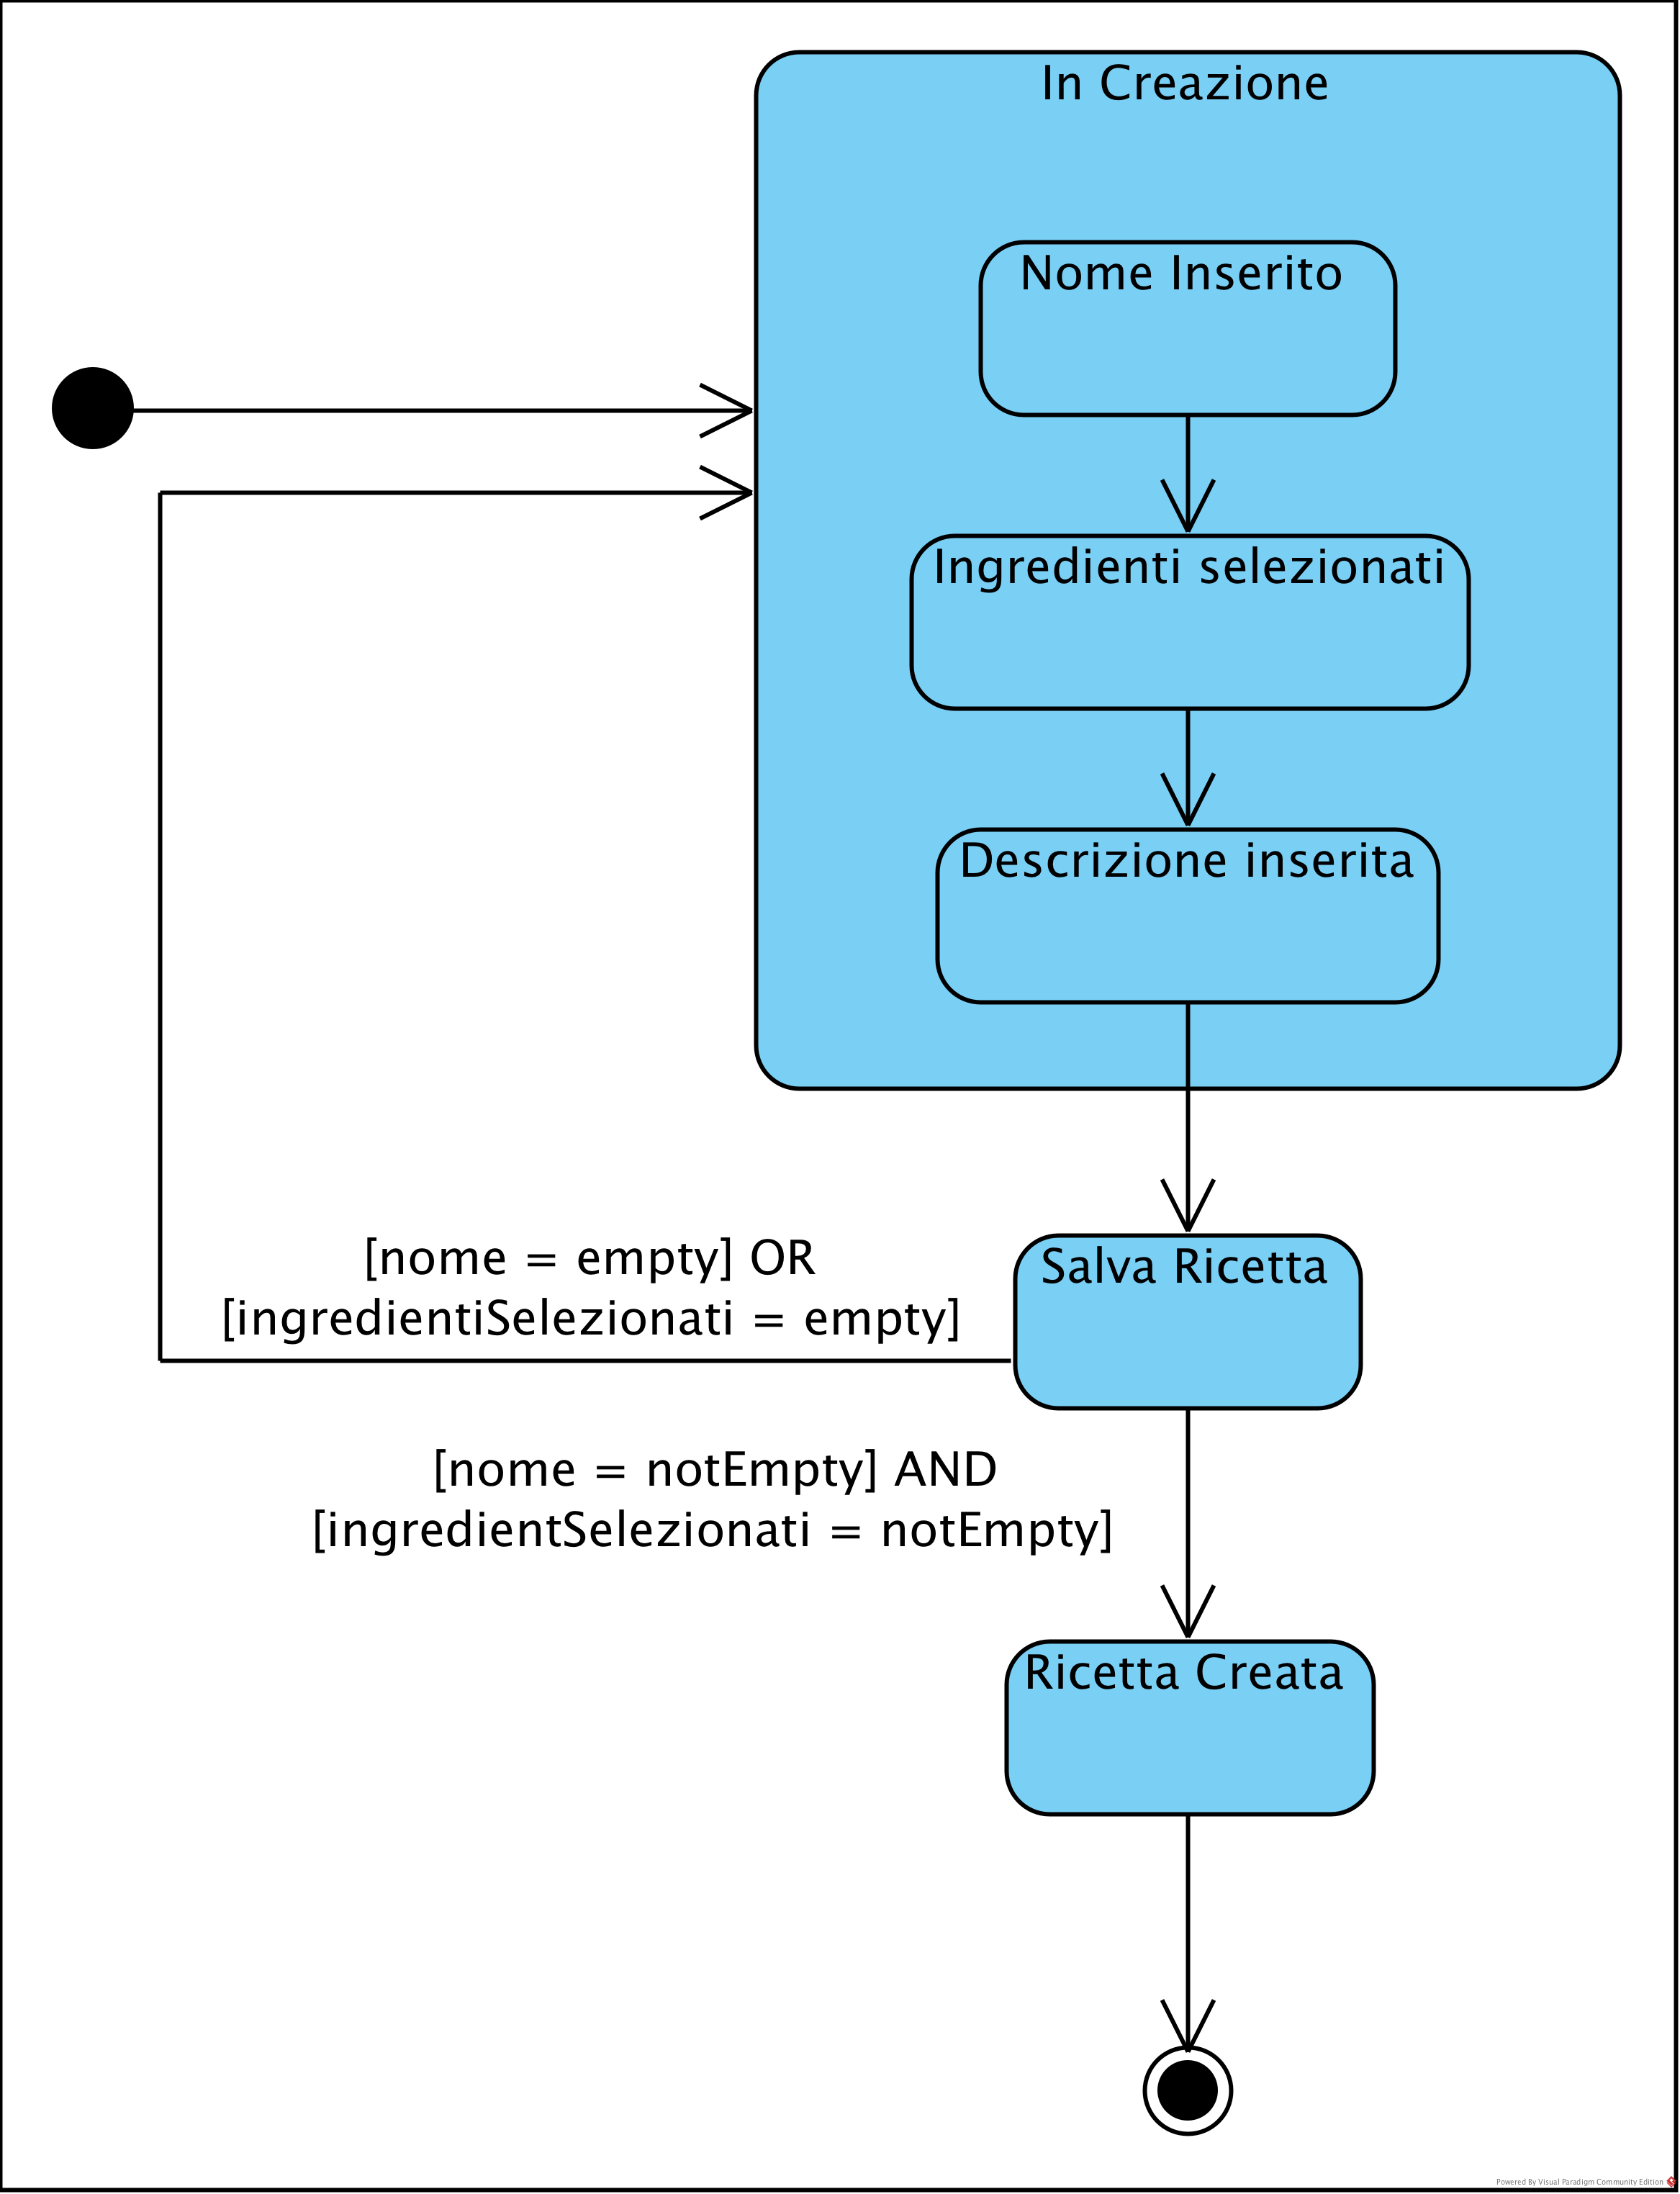
\includegraphics[height=400px]{diagramma_macchina_stati_addRecipe.png}
\caption{\label{fig:diagramma_macchina_a_stati}Diagramma macchina a stati per addRecipe}
\end{figure}


\subsection{Diagramma di attività}
\begin{figure}[H]
\centering
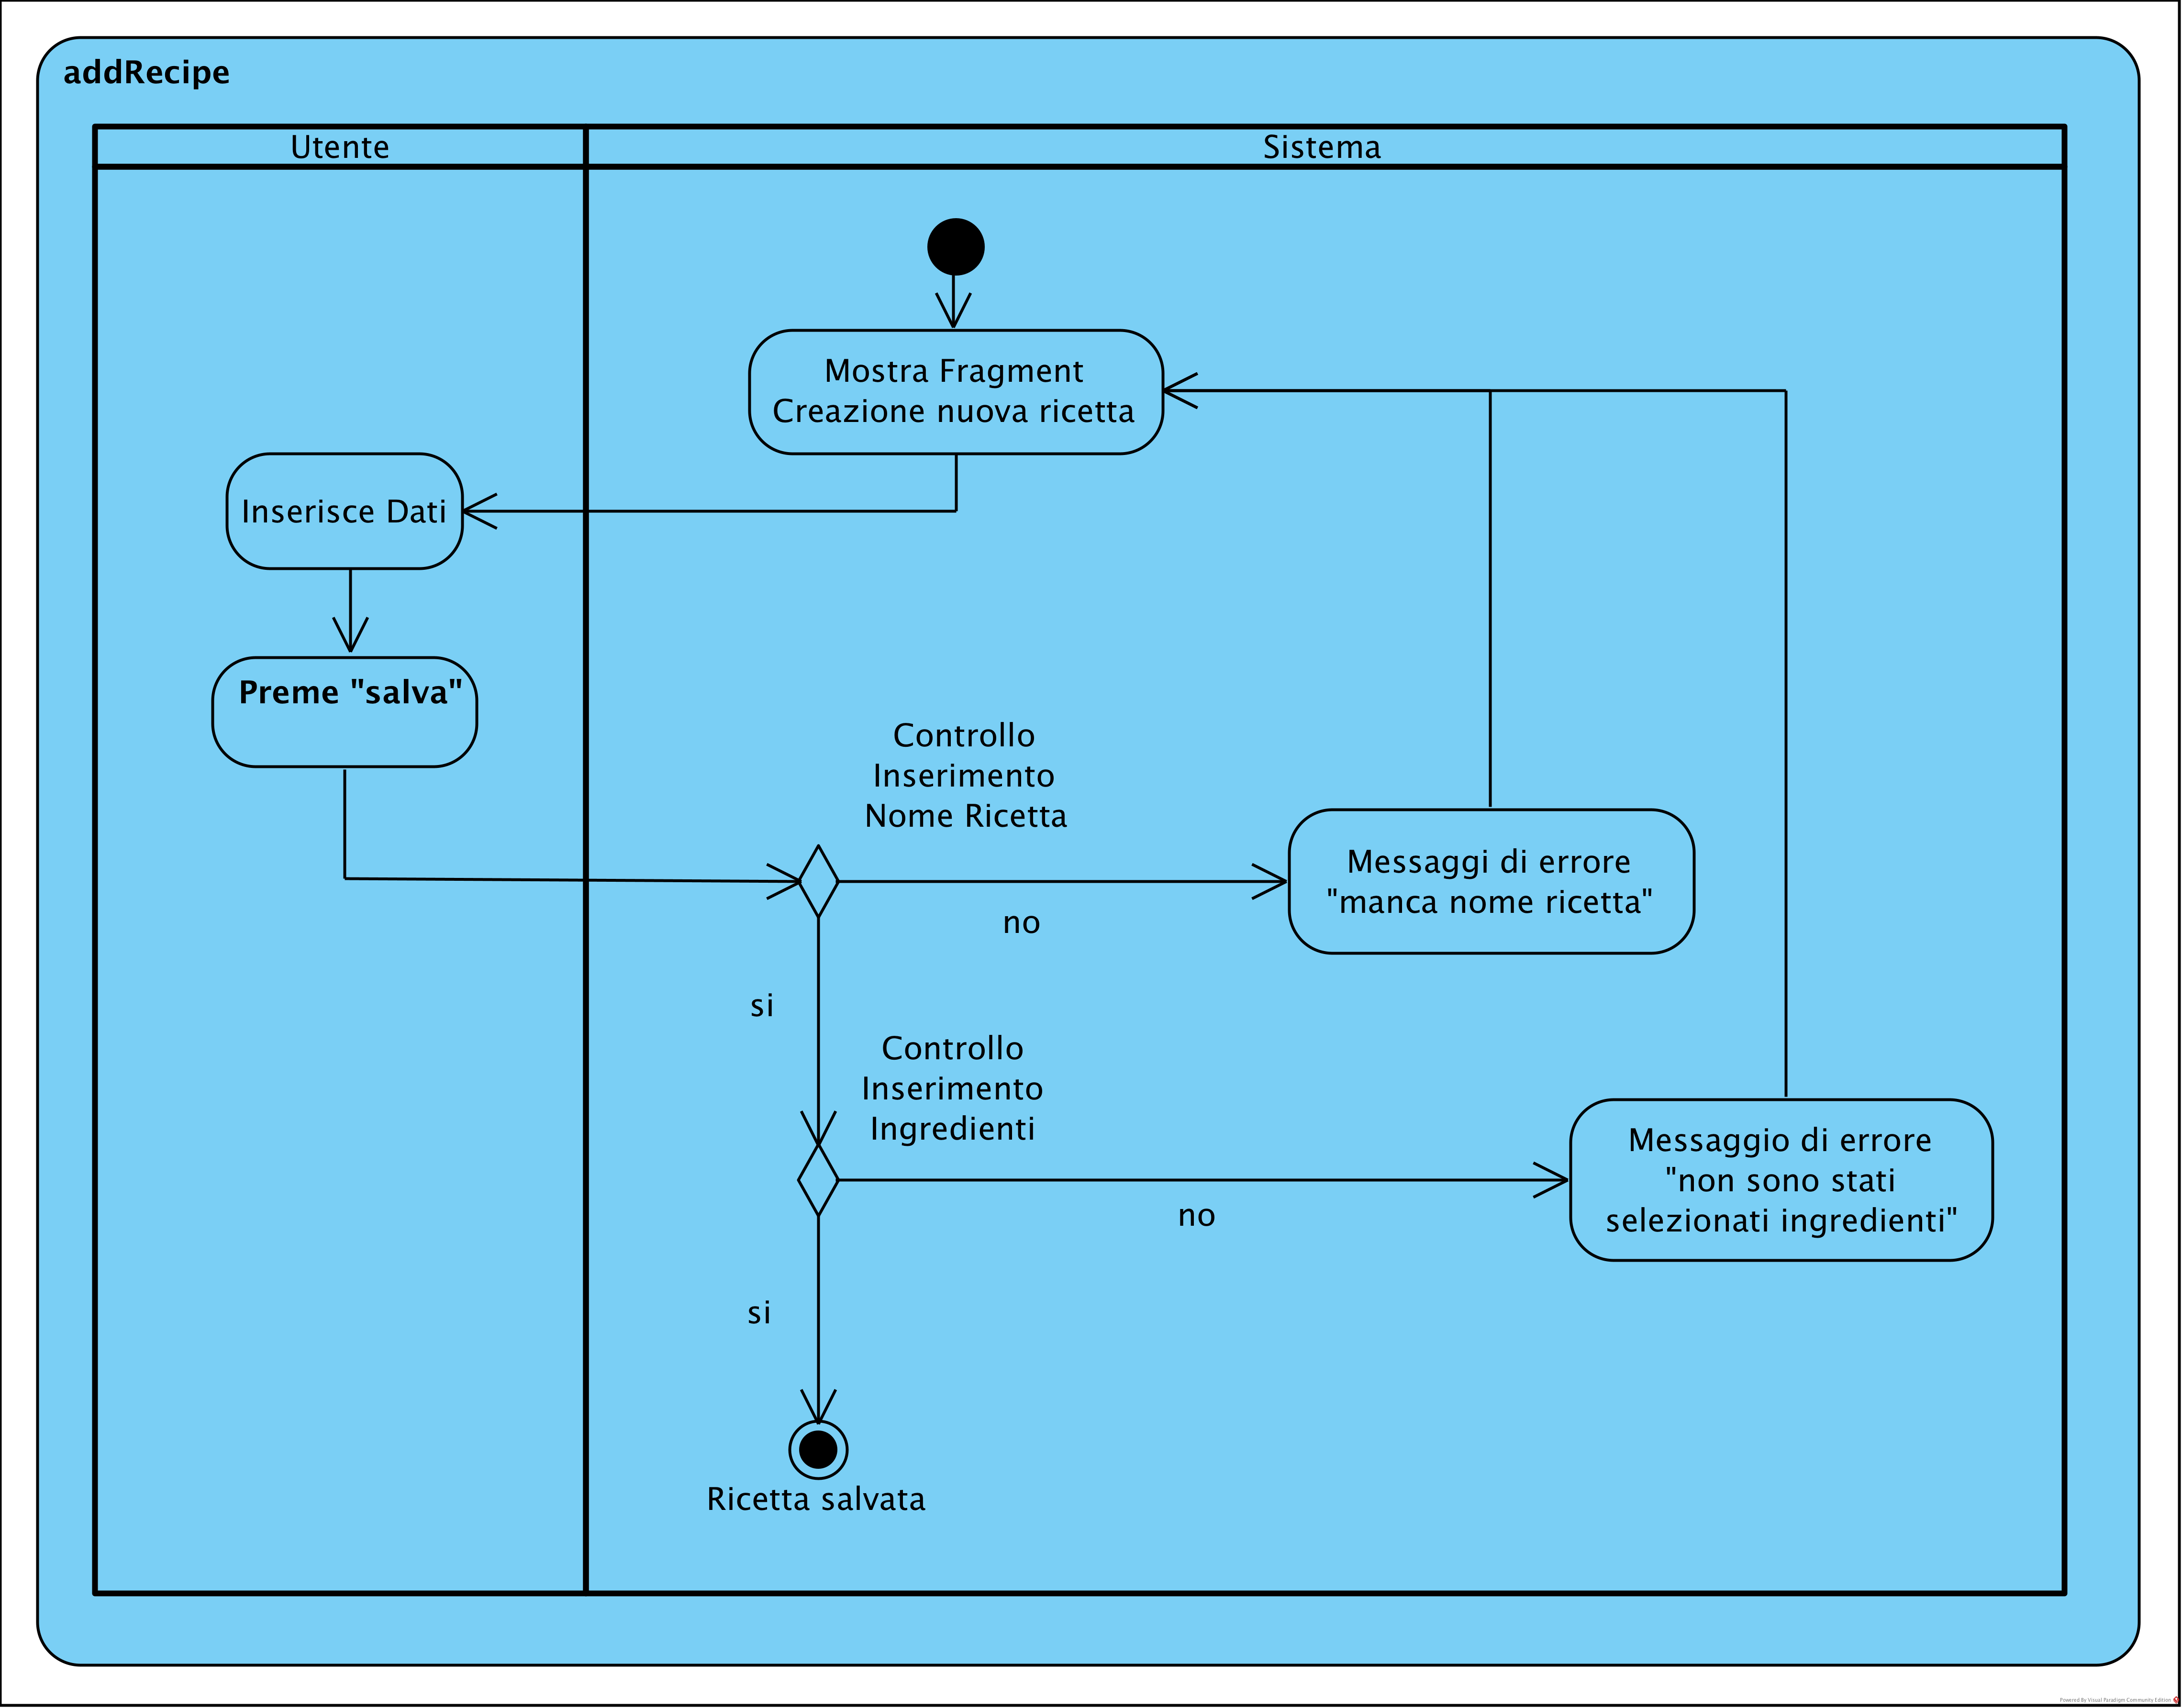
\includegraphics[width=440px]{diagramma_attivita_addRecipe.png}
\caption{\label{fig:diagramma_di_attivita}Diagramma di attività per addRecipe}
\end{figure}


\subsection{Diagramma dell'architettura software}
\begin{figure}[H]
\centering
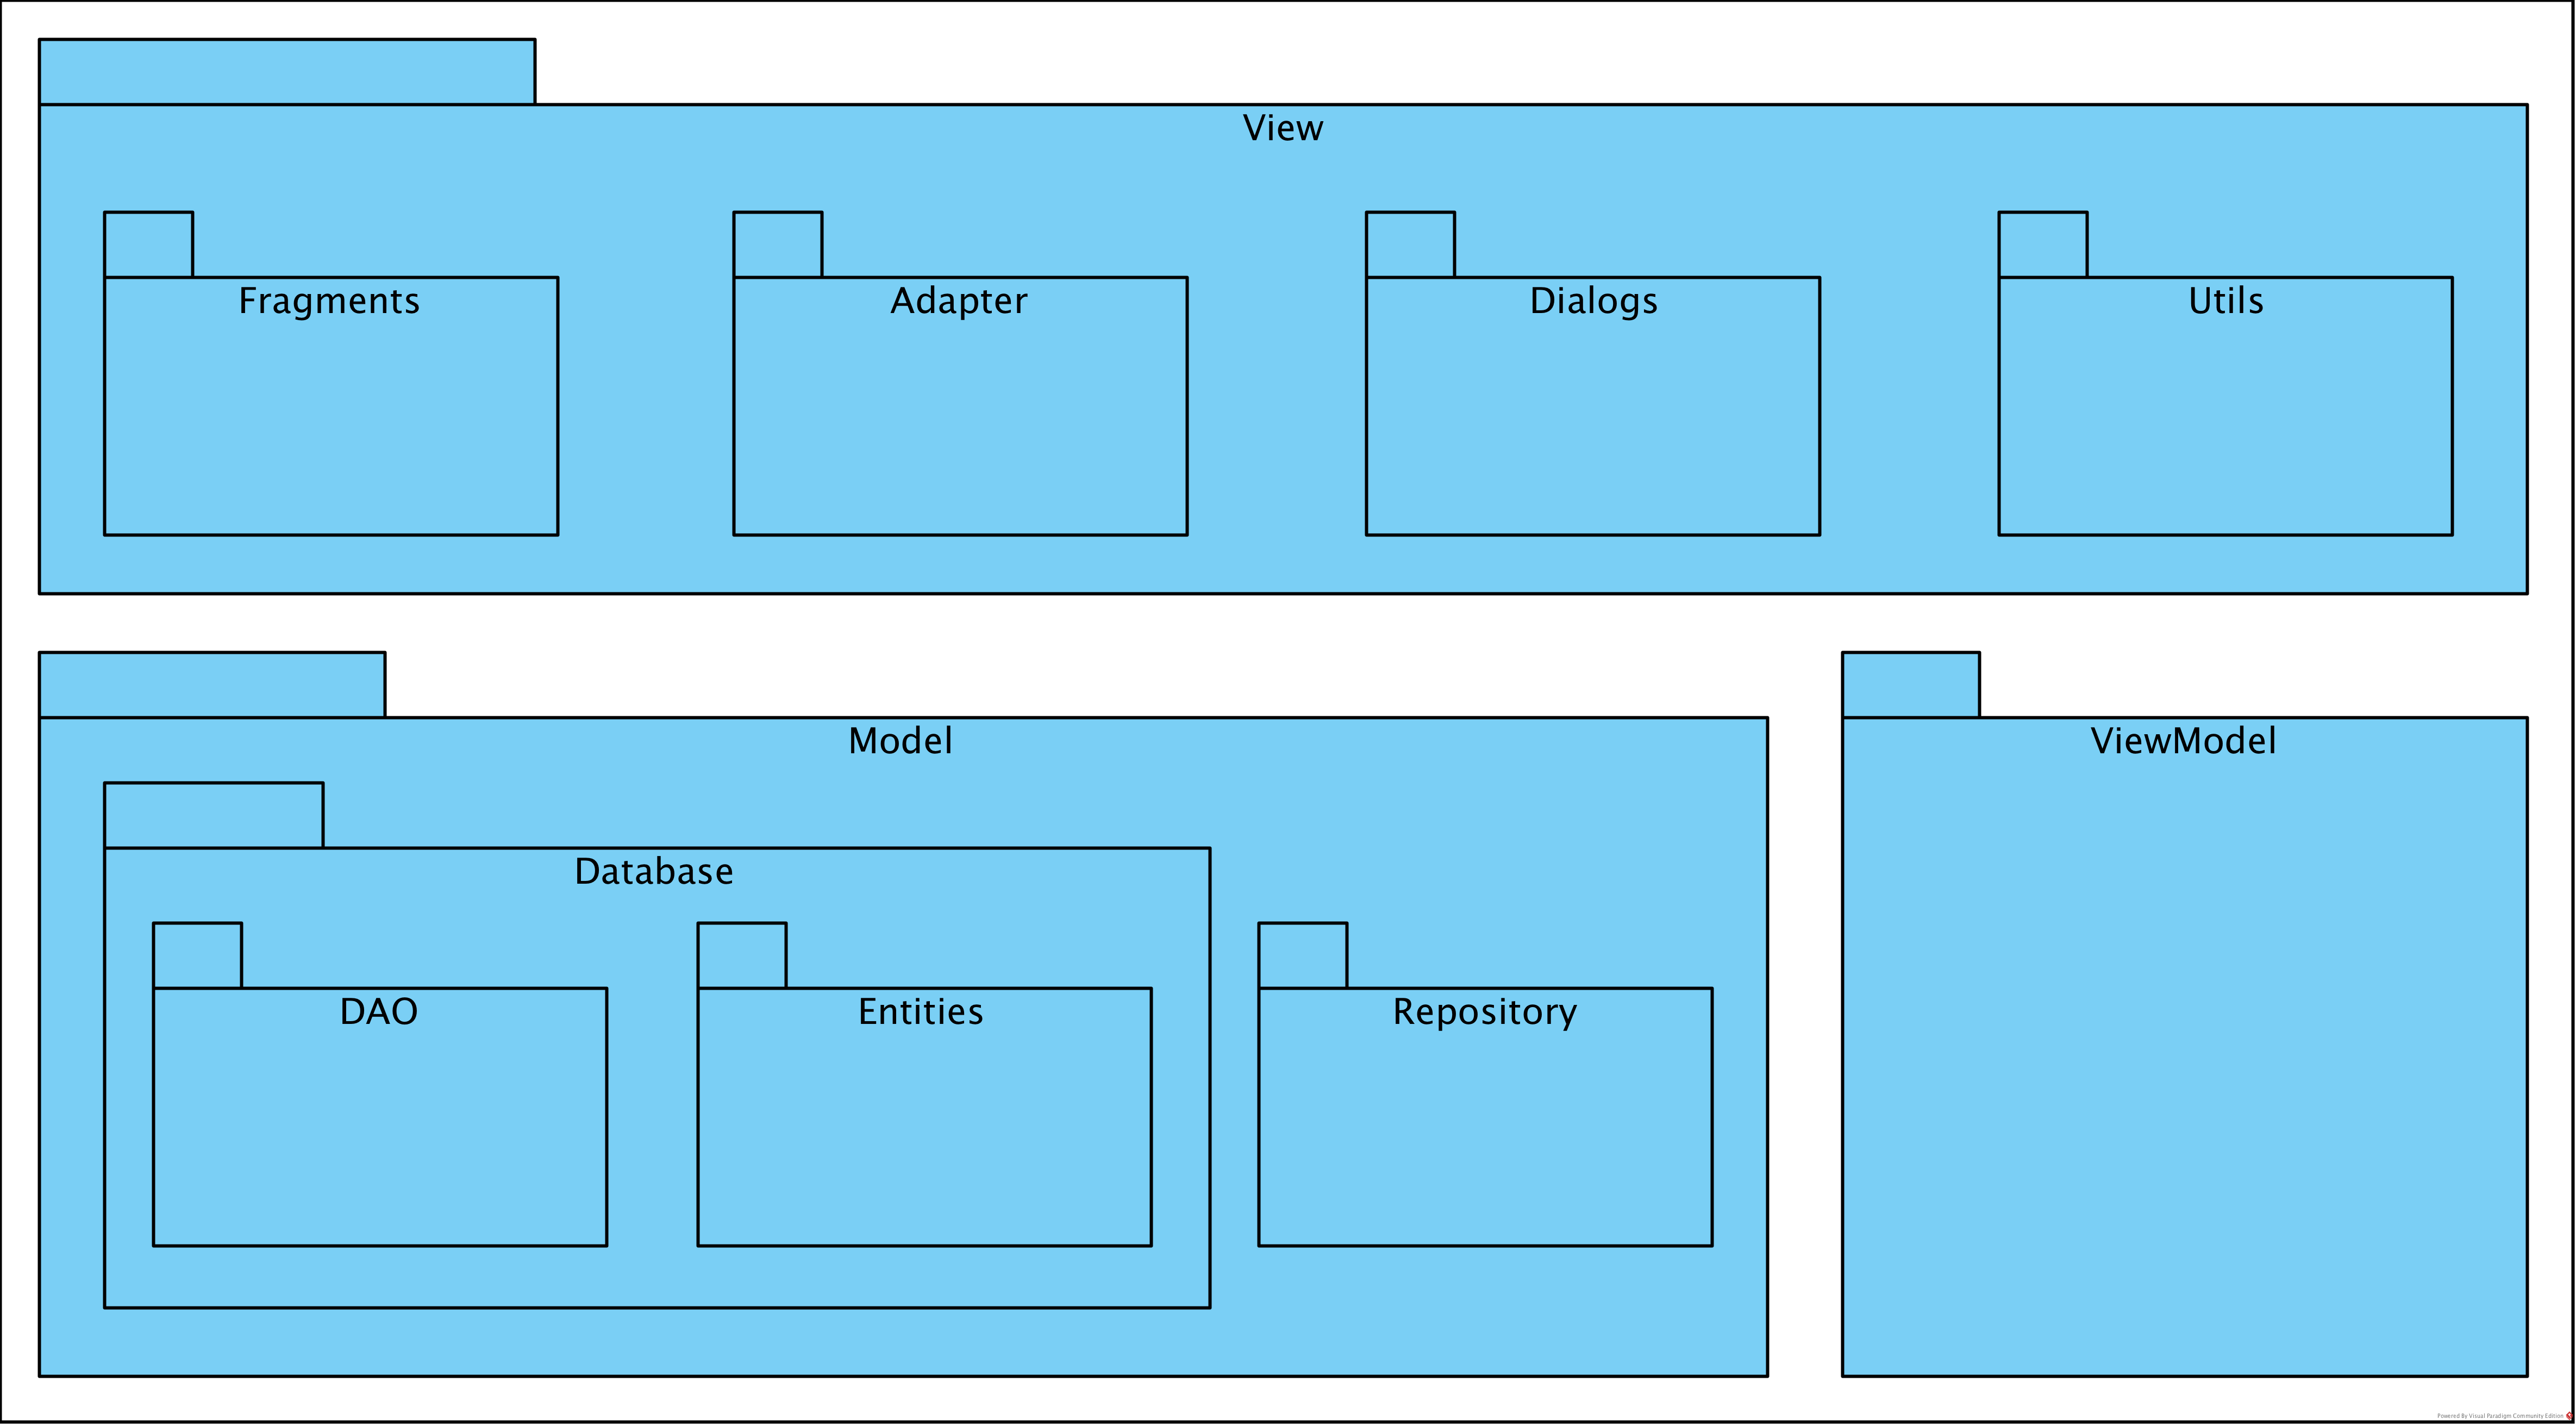
\includegraphics[width=440px]{diagramma_architettura.png}
\caption{\label{fig:diagramma_architettura_software}Diagramma dell'architettura software}
\end{figure}


%%%%%%%%%%%%%%%%%%%%%%%%%%%%%%%%%%%%%%%%%%%%%%%%%%%%%%%%%%%%%%%%%%%%%%%%%%%%%%%%%%%%%%%
\newpage
\section{Implementazione}

\subsection{Design Pattern }
I design pattern utilizzati fanno riferimento a \cite{martin2000design}

\subsubsection{Observer}
Il pattern Observer è presente tramite l'utilizzo di LiveData. Oltre a notificare le view degli aggiornamenti relativi a ricette, ingredienti ed equipaggiamento, i LiveData sono lifecyle-aware, ovvero rispettano il ciclo di vita delle varie componenti dell'applicazione (come activity o fragment) andando ad aggiornare solamente le componenti in uno stato attivo.

\subsubsection{Singleton}
Il pattern Singleton è stato utilizzato per avere una singola istanza del database all'interno dell'applicazione.

\subsection{Pattern Architetturali}
I pattern architetturali utilizzati fanno riferimento a quelli presentati da Fowler \cite{fowler2012patterns}.

\subsubsection{Model View Viewmodel}
Il pattern architetturale MVVM è una variante del pattern Presentation Model Design di Martin Fowler \cite{fowler2012patterns}. Si compone di tre parti principali: il model (modello), la view (vista) e il view model (modello della vista) a cui si accosta il meccanismo di binding per matenere sincronizzati questi ultimi due. Nello sviluppo dell'applicazione questo pattern è stato di fondamentale importanza per gestire la logica delle view attraverso il view model.


\subsection{Design Principle}
I design principle utilizzati fanno riferimento a \cite{martin2000design}

\subsubsection{Acyclic Dependencies Principle (ADP)}
É stato seguito questo design principle con l'intento di mantenere i package privi di cicli.
 

\subsection{Antipattern strutturali}
Non sono stati riscontati Antipattern strutturali.


\subsection{Mockup}
\begin{figure}[H]
\centering
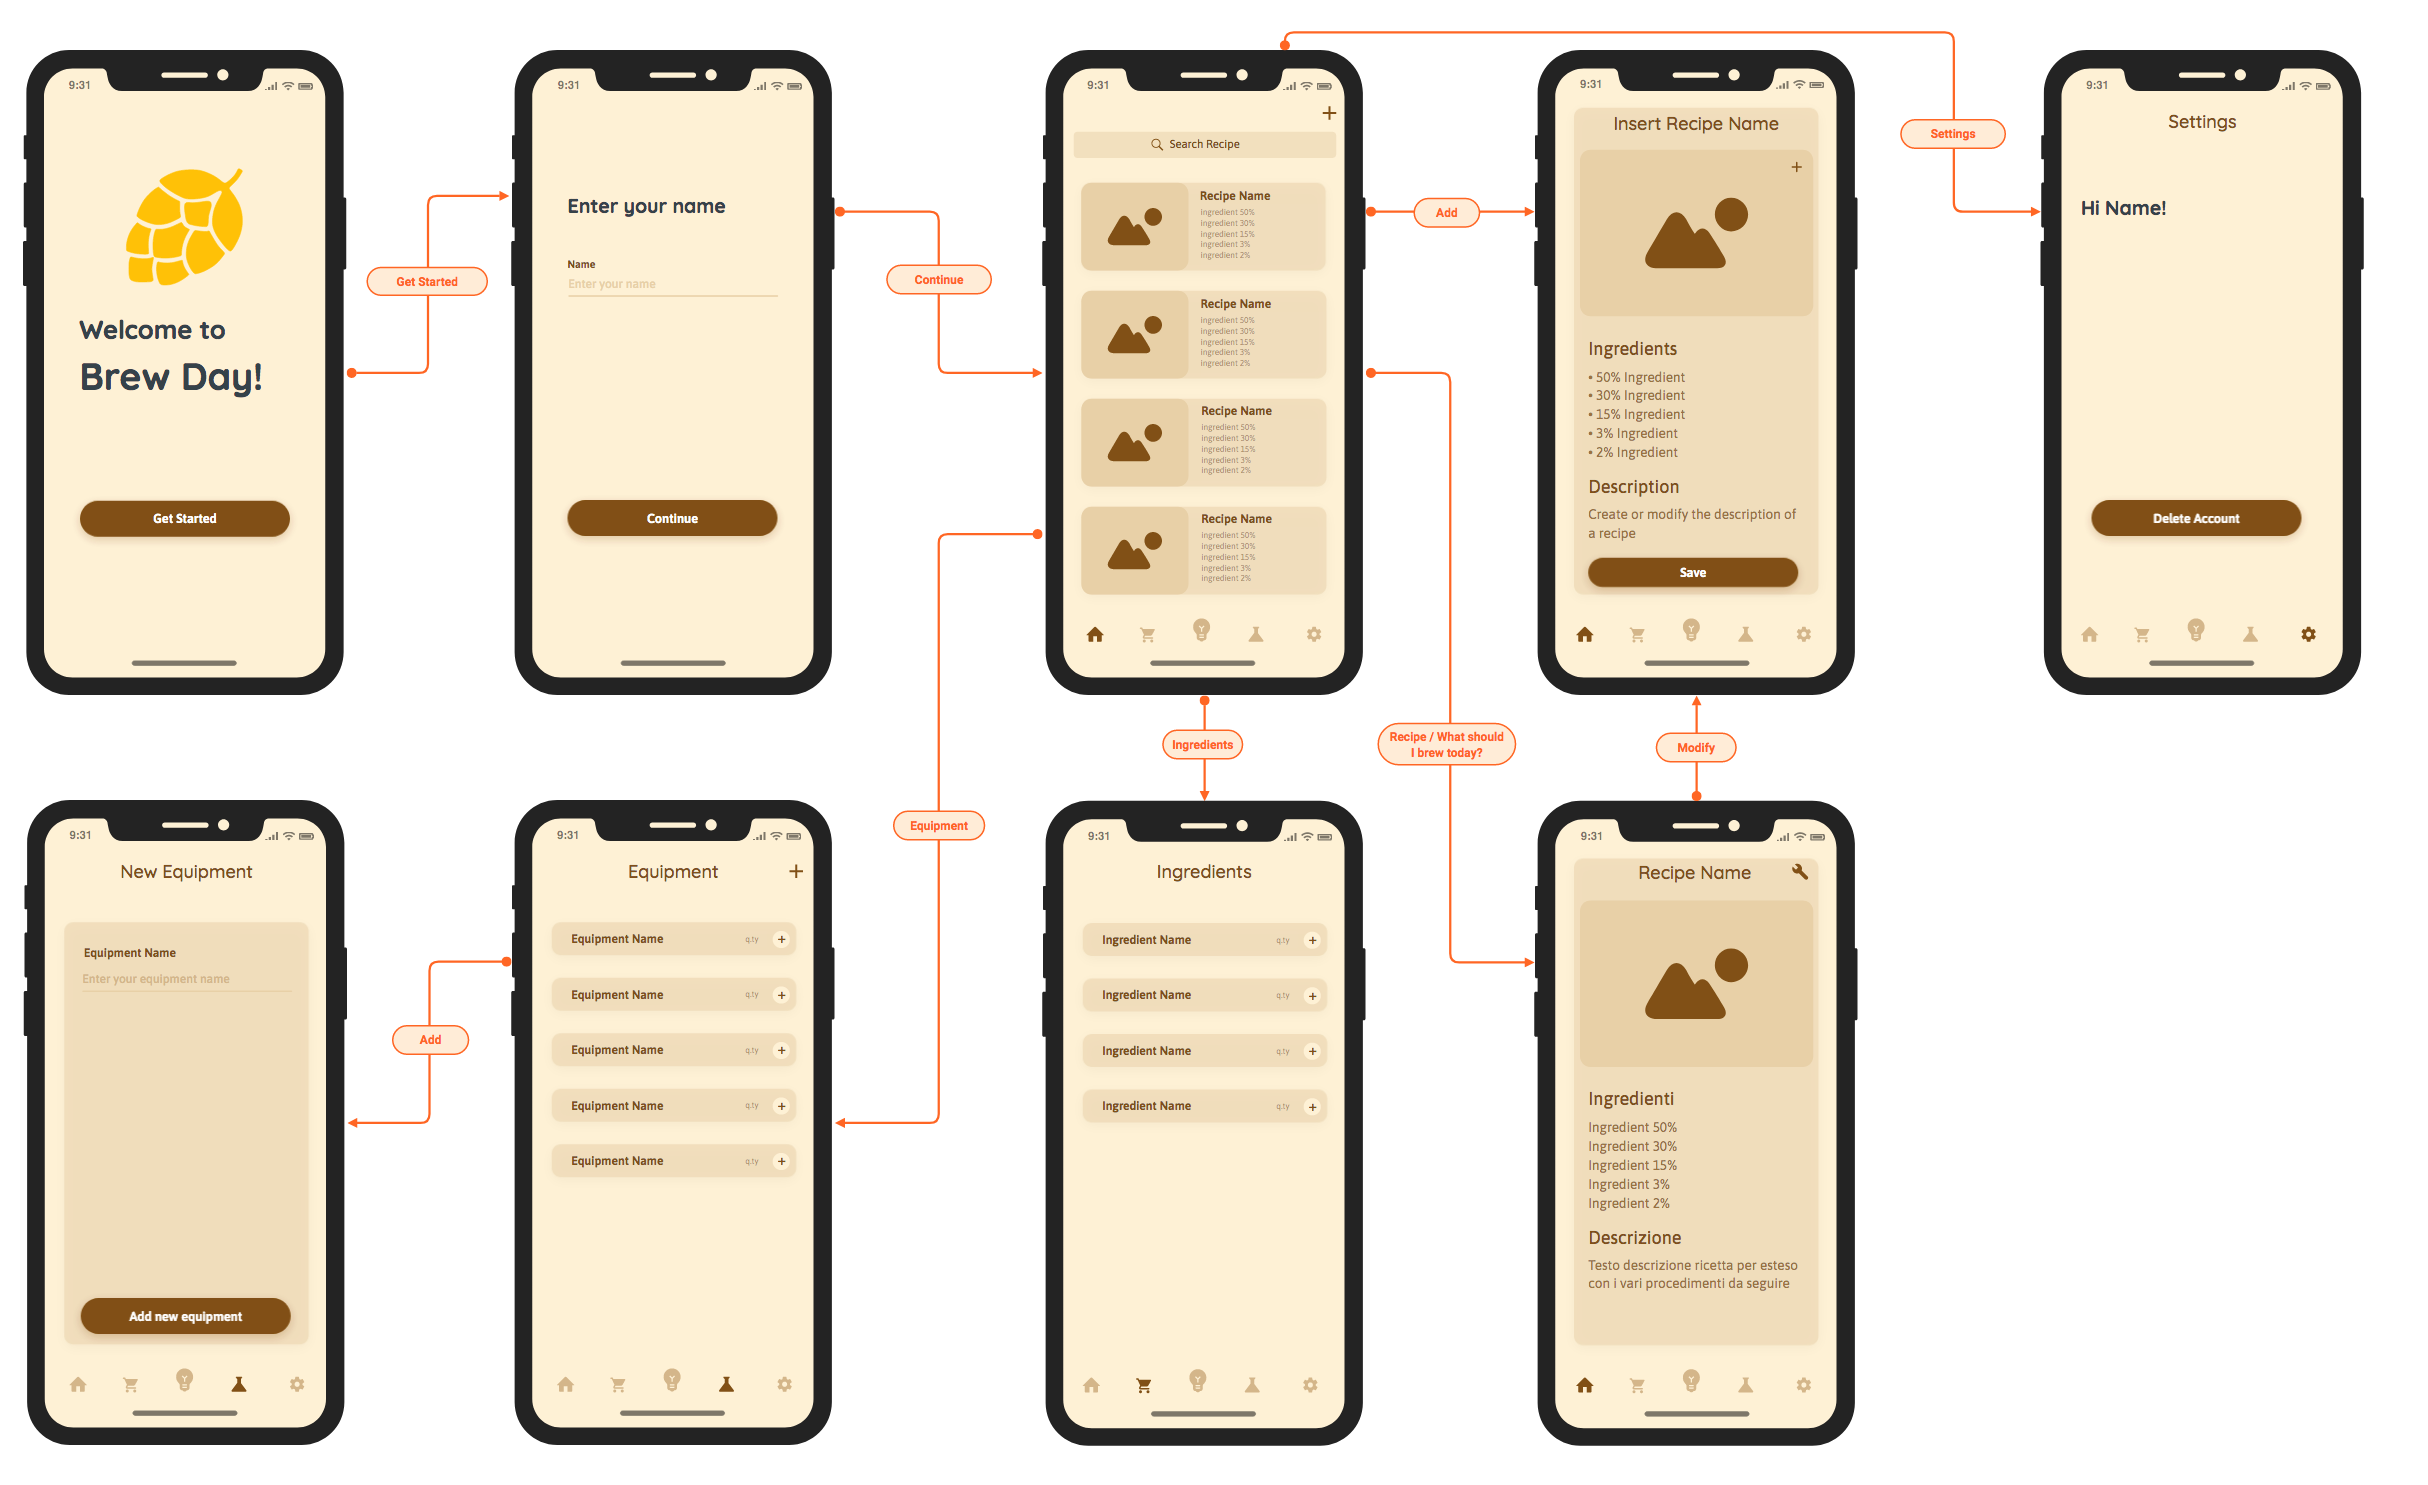
\includegraphics[width=450px]{mockup.png}
\caption{\label{fig:mockup}Mockup iniziale dell'applicazione}
\end{figure}


\subsection{Logo}
Per il logo dell'applicazione è stata scelta l'immagine di un luppolo stilizzato.
\begin{figure}[H]
\centering

\includegraphics[width=50px]{logo.png}
\caption{\label{fig:logo}Logo dell'applicazione}
\end{figure}


\subsection{Palette}
A partire dal logo è stata definita la palette di colori utilizzati, prediligendo tonalità chiare per lo sfondo e tonalità scure per il testo.
\begin{figure}[H]
\centering
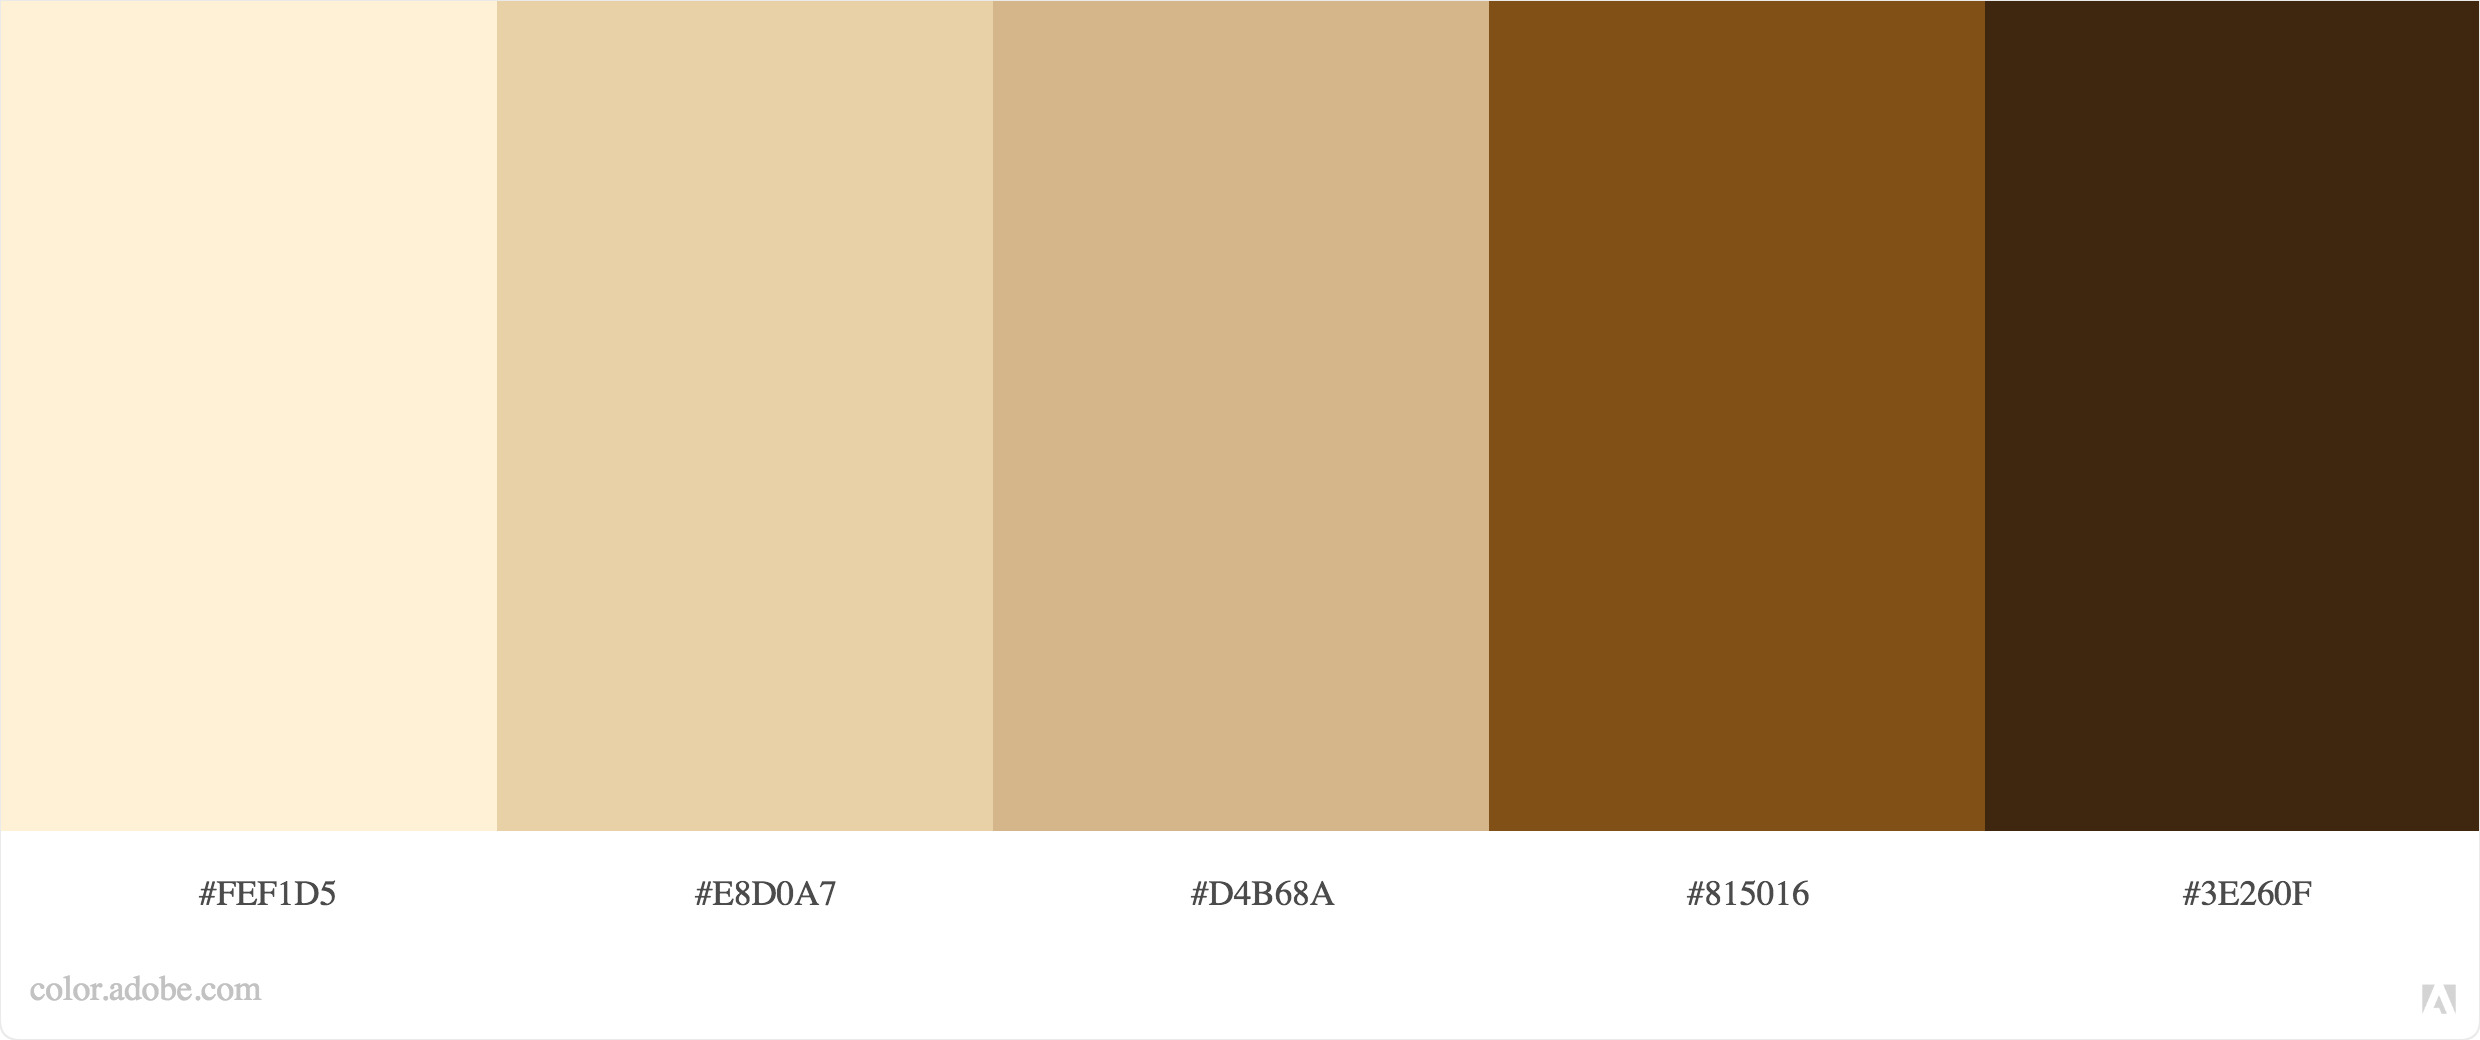
\includegraphics[height=100px]{palette.jpeg}
\caption{\label{fig:palette}Palette scelta per l'applicazione}
\end{figure}



%%%%%%%%%%%%%%%%%%%%%%%%%%%%%%%%%%%%%%%%%%%%%%%%%%%%%%%%%%%%%%%%%%%%%%%%%%%%%%%%%%%%%%%
\newpage
\section{Tecnologie utilizzate}

\subsection{Room}
L'utilizzo della libreria Room ha permesso un facile mantenimento del database. \newline
In particolare sono state create le diverse Entità e i vari DAO (data access object) ad esse associati.
\begin{figure}[H]
\centering
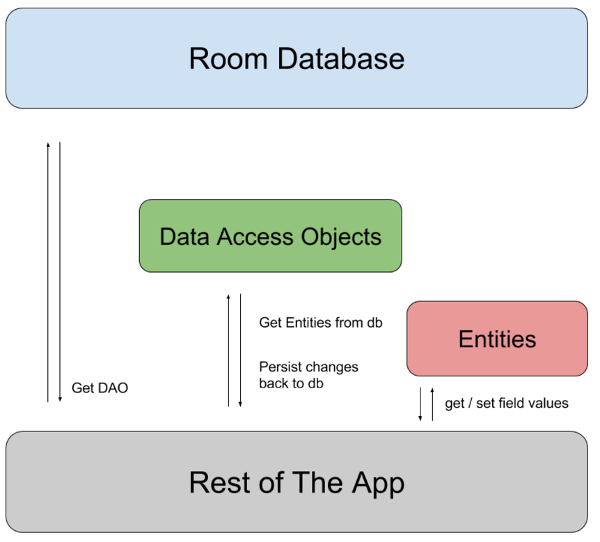
\includegraphics[height=250px]{room.png}
\caption{\label{fig:room}Schema sintetico sul funzionamento di Room}
\end{figure}


\subsection{Espresso}
Espresso è un framework usato nella creazione di test automatizzati per l'interfaccia utente (UI) di Android che fa parte dell'Android Testing Support Library.\newline
I test Espresso possono essere eseguiti sul device effettivo oppure su un emulatore, simulando il reale comportamento di un utente.


\subsection{Github}
Durante lo sviluppo del progetto sono state utilizzate diverse funzionalità offerte da github nell'ambito dell'organizzazione del lavoro. In particolare è stato utilizzato il sistema delle issue e delle pull request. Il primo per tenere traccia delle nuove features (alcune di queste sono state anche discusse, sempre all'interno della sezione issue) da aggiungere e dei bug riscontrati, mentre il secondo per fare la merge dei vari branch nel master con l'intento di produrre un lavoro più "pulito". In aggiunta si è cercato di utilizzare nomi dei branch e messaggi di commit inerenti alle modifiche apportate.


\subsection{Sonarcloud}
L'utilizzo del tool SonarCloud ha permesso di controllare la qualità del codice scritto, in particolare ha permesso di individuare e risolvere alcuni code smell minori.
Il controllo di SonarCloud è stato applicato unicamente al branch master.
\begin{figure}[H]
\centering
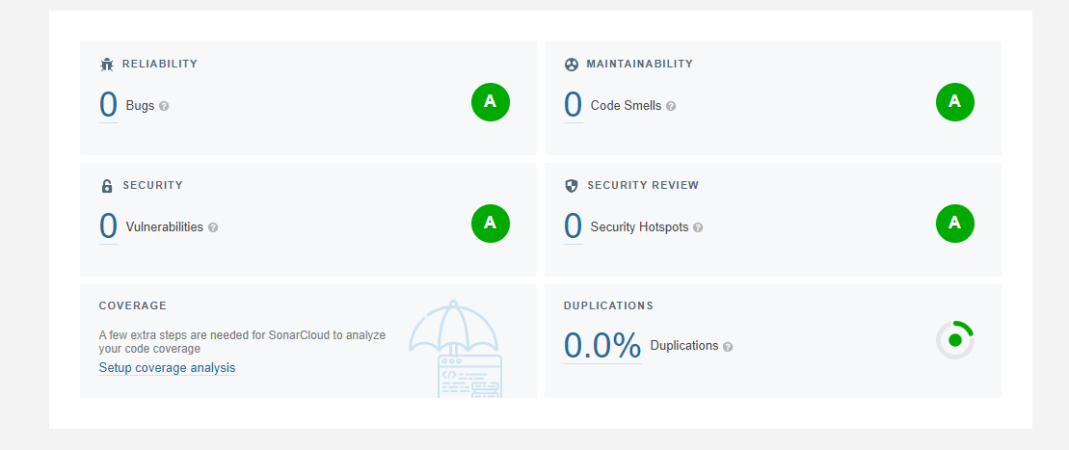
\includegraphics[width=400px]{sonarcloud.png}
\caption{\label{fig:sonarcloud}Analisi di SonarCloud in data 31.01.2022}
\end{figure}



%%%%%%%%%%%%%%%%%%%%%%%%%%%%%%%%%%%%%%%%%%%%%%%%%%%%%%%%%%%%%%%%%%%%%%%%%%%%%%%%%%%%%%%
\newpage
\section{Istruzioni}

\subsection{Installazione}
É possibile installare il file eseguibile APK direttamente su un dispositivo Android (versione 8.0 o successive), dando in precedenza i permessi per poter installare applicazioni non provenienti dal PlayStore.\newline
In alternativa è possibile usare direttamente l'emulatore presente all'interno dell'IDE Android Studio.
\begin{itemize}
    \item[-] Installare Android Studio
    \item[-] Scaricare il codice dell'applicazione da git
    \begin{itemize}
        \item[-] Get from VCS
        \item[-] Inserire dati di accesso
        \item[-] Inserire link al repository
        \begin{itemize}
            \item[  ]https://github.com/UnimibSoftEngCourse2022/progetto-birra-1-beer2beer.git
            \item[  ]git@github.com:UnimibSoftEngCourse2022/progetto-birra-1-beer2beer.git
        \end{itemize}
    \end{itemize}
    \item[-] Creare un device per l'emulatore
    \begin{itemize}
        \item[-] Tools \textgreater \space Device Manager
        \item[-] Virtual \textgreater \space Create device
        \item[-] Scegliere un dispositivo a scelta (scegliere una versione di android 8.0 o successive)
    \end{itemize}
    \item[-] Assicurarsi di aver selezionato il dispositivo appena creato e premere sulla freccia verde "play" 
\end{itemize}

\subsection{Utilizzo}
L'applicazione è pronta all'uso.\newline
Una volta installata e aperta verrà visualizzata una schermata di benvenuto. Procedendo verrà chiesto di inserire un nome, dopodiché ci si troverà nella homepage.\newline
L'applicazione permette di aggiungere nuovi equipaggiamenti ed eventualmente modificarli (una volta creati) scegliendo per ognuno un nome, la categoria di appartenenza e la capacità in litri. Inoltre è possibile eliminare un equipaggiamento facendo swipe a sinistra.\newline
Gli ingredienti presenti nell'applicazione sono predefiniti e inizialmente settati a 0. É possibile modificare manualmente il loro valore nell'apposita sezione.\newline
Per quanto riguarda le ricette è possibile aggiungerne di nuove, selezionando un titolo, gli ingredienti e una descrizione facoltativa. Una volta creata una ricetta è possibile cancellarla dalla homepage facendo swipe a sinistra. Cliccando sulla ricetta, invece, è possibile visualizzare la ricetta completa di dettagli (ingredienti e descrizione) e le eventuali note aggiunte in precedenza. In particolare, ogni qual volta si aggiunge una nuova istanza della ricetta (si prepara una ricetta) è possibile scrivere una nota.\newline
Premendo sul tasto centrale del menu verrà mostrata una ricetta che risponde alla funzionalità "What should I brew today?".\newline
Infine, eliminando il proprio account dalle impostazioni, verranno eliminati tutti i dati presenti nel database dell'applicazione.



\newpage
\bibliographystyle{alpha}
\bibliography{sample}

\end{document}